%%%%%%%%%%%%%%%%%%%%%%%%%%%%%%%%%%%%%%%%
% datoteka diploma-vzorec.tex
%
% vzorčna datoteka za pisanje diplomskega dela v formatu LaTeX
% na UL Fakulteti za računalništvo in informatiko
%
% vkup spravil Gašper Fijavž, december 2010
% množica popravkov v januarju, februarju marcu 2011
% verzija 29. marec 2011

\documentclass[a4paper, 12pt]{book}

\usepackage[utf8x]{inputenc}   % omogoča uporabo slovenskih črk kodiranih v formatu UTF-8 
\usepackage{hyperref}
\usepackage[slovene,english]{babel}    % naloži, med drugim, slovenske delilne vzorce
\usepackage[pdftex]{graphicx}  % omogoča vlaganje slik različnih formatov 
\usepackage{fancyhdr}          % poskrbi, na primer, za glave strani
\usepackage{amssymb}           % dodatni simboli
\usepackage{amsmath}           % eqref, npr.
\usepackage{inconsolata}


\renewcommand{\baselinestretch}{1.3} % ustrezen razmik med vrsticami

%oznake strani
\renewcommand{\chaptermark}[1]%
{\markboth{\MakeUppercase{\thechapter.\ #1}}{}} \renewcommand{\sectionmark}[1]%
{\markright{\MakeUppercase{\thesection.\ #1}}} \renewcommand{\headrulewidth}{0.5pt} \renewcommand{\footrulewidth}{0pt} 
\fancyhf{}
\fancyhead[LE,RO]{\sl \thepage} \fancyhead[LO]{\sl \rightmark} \fancyhead[RE]{\sl \leftmark}

\newcommand{\BibTeX}{{\sc Bib}\TeX}

\newcommand{\autfont}{\Large}
\newcommand{\titfont}{\LARGE\bf}
\newcommand{\clearemptydoublepage}{\newpage{\pagestyle{empty}\cleardoublepage}}
\setcounter{tocdepth}{1}	      % globina kazala

% konstrukti
\newtheorem{izrek}{Izrek}[chapter]
%\newtheorem{trditev}{Trditev}[izrek]
\newenvironment{dokaz}{\emph{Dokaz.}\ }{\hspace{\fill}{$\Box$}}

\begin{document}
\selectlanguage{slovene}
\frontmatter
\setcounter{page}{1} %
\renewcommand{\thepage}{}       % preprecimo težave s številkami strani v kazalu 

%%%%%%%%%%%%%%%%%%%%%%%%%%%%%%%%%%%%%%%%
%naslovnica
 \thispagestyle{empty}%
   \begin{center}
    {\large\sc Univerza v Ljubljani\\%
      Fakulteta za računalništvo in informatiko}%
    \vskip 10em%
    {\autfont Anže Pečar\par}%
    {\titfont Medplatformni razvoj grafično intenzivnih aplikacij \par}%
    {\vskip 2em \textsc{DIPLOMSKO DELO\\[2mm] 
    UNIVERZITETNI ŠTUDIJSKI PROGRAM RAČUNALNIŠTVO IN INFORMATIKA}\par}%
    \vfill\null%
    {\large \textsc{Mentor}: doc.\ dr.  Matjaž Kukar\par}%
    {\vskip 2em \large Ljubljana 2013 \par}%
\end{center}
% prazna stran
\clearemptydoublepage

%%%%%%%%%%%%%%%%%%%%%%%%%%%%%%%%%%%%%%%%
%copyright stran
\thispagestyle{empty}
\vspace*{8cm}
{\small \noindent
Rezultati diplomskega dela so intelektualna lastnina avtorja in Fakultete za ra\-ču\-nal\-niš\-tvo in informatiko Univerze v Ljubljani. 
Za objavljanje ali izkoriščanje rezultatov di\-plom\-ske\-ga dela je potrebno pisno soglasje avtorja, Fakultete za ra\-ču\-nal\-niš\-tvo in 
informatiko ter mentorja.}



\begin{center} 
\mbox{}\vfill
\emph{Besedilo je oblikovano z urejevalnikom besedil \LaTeX.} 
\end{center}
% prazna stran
\clearemptydoublepage

%%%%%%%%%%%%%%%%%%%%%%%%%%%%%%%%%%%%%%%%
% stran 3 med uvodnimi listi
\noindent
Namesto te strani {\bf vstavite} original izdane teme diplomskega 
dela s podpisom mentorja in dekana ter žigom fakultete, ki ga diplomant
dvigne v študent\-skem referatu, preden odda izdelek v vezavo!

% prazna stran
\clearemptydoublepage

%%%%%%%%%%%%%%%%%%%%%%%%%%%%%%%%%%%%%%%%
% izjava o avtorstvu
\vspace*{1cm}
\begin{center} 
{\Large \textbf{\sc Izjava o avtorstvu diplomskega dela}}
\end{center}

\vspace{1cm}
\noindent Spodaj podpisani Anže Pečar,
z vpisno številko \textbf{63060257}, sem avtor  diplomskega dela z naslovom:
   
\vspace{0.5cm}
\emph{Medplatformni razvoj grafično intenzivnih aplikacij}

\vspace{1.5cm}
\noindent S svojim podpisom zagotavljam, da:
\begin{itemize}
	\item sem diplomsko delo izdelal samostojno pod mentorstvom 
		doc.\ dr.\ Matjaža Kukarja,

	\item	so elektronska oblika diplomskega dela, naslov (slov., angl.), povzetek (slov., angl.) ter ključne besede (slov., angl.) identični s tiskano obliko diplomskega dela
	\item soglašam z javno objavo elektronske oblike diplomskega dela v zbirki ''Dela FRI''.
\end{itemize}

\vspace{1cm}
\noindent V Ljubljani, dne 11. januarja 2013 \hfill Podpis avtorja:

% prazna stran
\clearemptydoublepage

%%%%%%%%%%%%%%%%%%%%%%%%%%%%%%%%%%%%%%%%
% zahvala
\thispagestyle{empty}\mbox{}\vfill\null\it%
Zahvala
\rm\normalfont

% prazna stran
\clearemptydoublepage

%%%%%%%%%%%%%%%%%%%%%%%%%%%%%%%%%%%%%%%%
% posvetilo
\thispagestyle{empty}\mbox{}{\vskip0.20\textheight}\mbox{}\hfill\begin{minipage}{0.55\textwidth}%
Posvetilo% Svoji dragi Nataščici.
\normalfont\end{minipage}
 
% prazna stran
\clearemptydoublepage

%%%%%%%%%%%%%%%%%%%%%%%%%%%%%%%%%%%%%%%%
% kazalo
\def\thepage{}% preprecimo tezave s stevilkami strani v kazalu 
\tableofcontents{}


% prazna stran
\clearemptydoublepage

%%%%%%%%%%%%%%%%%%%%%%%%%%%%%%%%%%%%%%%%
% povzetek 
\addcontentsline{toc}{chapter}{Povzetek}
\chapter*{Povzetek}

V diplomskem delu smo naredili pregled metod za razvoj grafično intenzivnih aplikacij na različnih platformah. Raziskali smo možne platforme in si ogledali razlike med njimi. Poseben poudarek smo namenili mobilnim napravam. V nadaljevanju diplomskega dela smo si ogledali metode in orodja, s katerimi je možno premostiti razlike med platformami. Štiri metode smo opredelili bolj podrobno in za vsako od teh razvili testno aplikacijo. Raziskali smo tudi računanje na grafičnih procesnih enotah, saj lahko postane pomemben faktor pri razvoju medplatformnih aplikacij v prihodnosti. Ugotovili smo, da uporaba obravnavanih metod pohitri in poenostavi razvoj medplatformnih aplikacij.

\subsection*{Ključne besede:}

grafično intenzivne aplikacije, platforme, razvojna orodja, mobilne naprave, spletne tehnologije

% prazna stran
\clearemptydoublepage

%%%%%%%%%%%%%%%%%%%%%%%%%%%%%%%%%%%%%%%%
% abstract
\selectlanguage{english}
\addcontentsline{toc}{chapter}{Abstract}
\chapter*{Abstract}


We have investigated methods of developing cross-platform graphics-intense applications. We have researched different platforms and pointed out differences between them. Mobile platforms have received special attention. We have taken a look into methods and tools for overcoming differences between the platforms. We studied four methods more thoroughly and implemented test applications for each of those. Additionaly, we have researched computing on graphics processing units as this may become an important factor for developing cross-platform applications in the future. We concluded that cross-platform applications can be developed faster and easier by exerting the discussed methods.

\subsection*{Keywords:}

graphics-intensive applications, platforms, development tools, mobile devices, web technologies 

\selectlanguage{slovene}

\selectlanguage{slovene}
% prazna stran
\clearemptydoublepage

%%%%%%%%%%%%%%%%%%%%%%%%%%%%%%%%%%%%%%%%
\mainmatter
\setcounter{page}{1}
\pagestyle{fancy}



\chapter{Uvod}

Še pred nekaj leti je bilo poganjanje grafično intenzivnih aplikacij domena dragih delovnih postaj. Danes je tega zmožen vsak osebni računalnik in tudi naprave, ki jih prenašamo v žepih.

Zmogljive mobilne naprave postajajo vse bolj vsakdanje. Pametni telefoni imajo v sebi več procesorske moči, kot namizni računalniki izpred parih let. Poleg procesorske moči praviloma vsebujejo tudi grafične procesne enote, ki jih razvijalci lahko izkoristijo za razvoj grafično intenzivnih aplikacij. Poleg telefonov pa so se pojavili tudi tablični računalniki, ki imajo praviloma še boljše karakteristike kot pametni telefoni. 

Med posameznimi proizvajalci telefonov in tablic obstajajo velike razlike v razvojnem okolju. Vsak izmed mobilnih operacijskih sistemov uporablja drug programski jezik za razvoj domorodnih aplikacij pa tudi pri knjižnicah se pojavljajo razlike (npr. OpenGL ES, Direct3D). Razvoj grafične aplikacije, ki bi jo napisali enkrat in bi delovala povsod, je tako skorajda nemogoč.

Problem postane še težji, če želimo poleg vseh mobilnih naprav podpreti še namizne računalnike. Sedaj imamo poleg različnih programskih jezikov in knjižnic, še različne možnosti interakcije z uporabnikom - vnos z dotikom na mobilnih napravah in vnos z miško in tipkovnico na namiznih računalnikih.

\section{Potek diplomske naloge}

Cilj diplomske naloge je pregledati in preizkusiti možnosti za premostitev razlik med različnimi platformami. Na začetku si bomo ogledali različne platforme, njihove razlike in skupne točke. Osredotočili se bomo na mobilne platforme, vendar se bomo dotaknili tudi namiznih računalnikov in računalnikov na eni sami ploščici.

V nadaljevanju diplomske naloge si bomo ogledali nekatera odprtokodna in plačljiva orodja za premostitev razlik med platformami. Preučili bomo spletne tehnologije in orodja, ki temeljijo na prevodih med različnimi programskimi jeziki. Zanimale nas bodo metode, ki temeljijo na uporabi jezika C++, ter orodja, ki ponujajo celotno razvojno okolje. Ogledali si bomo tudi orodje, ki uporablja namenski programski jezik.

Ena izmed glavnih ovir pri razvoju grafično intenzivnih aplikacij s pomočjo spletnih tehnologij je hitrost izvajanja programa znotraj spletnega brskalnika. Zato bomo raziskali načine za pospešitev JavaScript izvorne kode.

Grafično intenzivne aplikacije za tekoče delovanje uporabljajo vedno višje stopnje paralelnosti. S tem razlogom si bomo ogledali procesiranje na grafičnih procesnih enotah.

V zadnjem delu diplomske naloge bomo opisali nekaj primerov grafično intenzivnih aplikacij, ki so bile razvite z namenom pokazati prednosti in slabosti uporabljenih orodij. Razložili bomo uporabljene metode, njihove prednosti in slabosti.

\chapter{Pregled platform za izvajanje grafično intenzivnih aplikacij}

Danes lahko grafično intenzivne aplikacije izvajamo na ogromnem naboru različnih naprav. Grafično pospešeno izrisovanje 3D objektov, ki je bilo še pred kratkim omejeno na namizne računalnike in še pred tem na drage delovne postaje, je sedaj možno tudi na mobilnih telefonih in grafičnih tablicah. Razvoj aplikacij za mobilne platforme je nekoliko bolj zahteven, saj moramo poleg okrnjenega nabora funkcionalnosti in slabše strojne zmogljivosti, paziti tudi na porabo baterije.

Omeniti moramo razliko med večplatformnim (angl. multi-platform) in medplatformnim (angl. cross-platform) razvojem aplikacij. Ker nismo našli točnih definicij teh dveh pojmov, se opiramo na sorodna pojma medjezično in večjezično (npr. iskanje). Medjezično iskanje je iskanje, pri katerem je naravni jezik iskalne zahteve lahko različen od jezika ali jezikov, v katerih je izražena vsebina dokumentov \cite{jezicno}. Podobno je lahko programski jezik, v katerem je napisana medplatformna aplikacija, različen od programskih jezikov, ki jih uporabljajo ciljne platforme. Večplatformna aplikacija je širši pojem, ki zajema medplatformne aplikacije in tudi aplikacije, ki so bile ročno prepisane v programske jezike posameznih ciljnih platform. Medplatformne aplikacije morajo imeti skupen vsaj del izvorne kode na vseh platformah. Če aplikacija temu pogoju ne ustreza, vendar še vseeno deluje na različnih platformah, rečemo, da je večplatforma.

\section{Namizni in prenosni računalniki}

Največ svobode pri razvoju grafično intenzivnih aplikacij je na voljo na namiznih računalnikih. Ti imajo na voljo najboljšo možno strojno opremo in tudi operacijski sistemi so zreli in dovršeni, saj so v razvoju že več deset let. Namizni računalniki nimajo tako strogih omejitev z velikostjo, kot mobilne naprave. Prav nič presenetljivo torej, da so grafično intenzivne aplikacije na tej platformi najbolj domače. 

Namizni računalniki uporabljajo drugačno arhitekturo centralne procesne enote kot večina mobilnih naprav. Procesorji v namiznih računalnikih so danes večinoma  zgrajeni s CISC arhitekturo (Intel, AMD), medtem ko mobilne naprave večinoma uporabljajo RISC arhitekturo in procesorje podjetij ARM in nVidia. Seveda obstajajo tudi izjeme, kot so na primer tablice s procesorji Intel Atom in PowerPC namizni računalniki.  

Namizni računalniki so bili zelo dolgo edina platforma, na kateri je bilo možno poganjati grafično intenzivne aplikacije. S pojavom grafičnih kartic se je zmanjšala obremenitev centralne procesne enote. Večji del operacij povezanih z izrisovanjem objektov na zaslonu, se danes izvaja na grafičnih procesnih enotah, ki imajo za ta namen visoko stopnjo paralelizma. 

Prenosni računalniki so po zmogljivosti podobni namiznim računalnikom. Za centralno procesno enoto uporabljajo tudi enako arhitekturo. Grafične procesne enote se na prenosnih računalnikih navadno sicer šibkejše kot na namiznih računalnikih, vendar so razlike minimalne. Razlog je v kompromisu med zmogljivostjo grafične kartice, porabo energije in prostorski omejenosti.

Na namiznih in kasneje na prenosnih računalnikih sta se v začetku 90. let pojavili dve knjižnici za delo s 3D grafiko: OpenGL in Direct3D. Obe ponujata programski vmesnik za komunikacijo z grafično procesno enoto, vendar so razlike med njima precejšne.

% http://en.wikipedia.org/wiki/Comparison_of_OpenGL_and_Direct3D

\subsection{OpenGL}

OpenGL je odprt standard, ki ga razvija skupina Khronos \cite{opengl}. Na voljo je na večini operacijskih sistemov (Windows, Mac OSX in Linux).

Programski vmesnik se je na začetku uporabljal predvsem za profesionalne aplikacije, kot je na primer AutoCAD in različne simulacije. Šele kasneje se je programski vmesnik razvil do te mere, da je bil uporaben tudi za druge namene.

Tekom let so izšle štiri večje posodobitve in kar nekaj manjših revizij. V času pisanja je najnovejša različica OpenGL 4.4. Podpora za programiranje grafičnega vhoda se je prvič pojavila pojavila v posodobitvi 3.0. Pred tem se je za izrisovanje uporabljal fiksen funkcijski cevovod. Prednost programiranega grafičnega vhoda je predvsem v večji fleksibilnosti, vendar za ceno večje kompleksnosti. OpenGL za vgrajene sisteme (OpenGL ES) je v prvi verziji uporabljal fiksen funkcijski cevovod, v reviziji 2.0 pa ga je zamenjal programiran vhod. 

OpenGL je implementiran v gonilniku za zaslon in vsak proizvajalec grafičnih kartic mora v gonilnike za grafično kartico dodati podporo. Problem s tem principom je, da se vmesnik nekoliko razlikuje med različnimi proizvajalci grafičnih kartic. Tudi programski jeziki za pisanje programov na grafični kartici in njihovi prevajalniki so si med seboj lahko malce različni.

Dolgo časa so obstajale tudi razširitve, ki so bile na voljo samo na določenih grafičnih karticah. Proizvajalci grafičnih kartic so na ta način želeli izkazati superiornost, saj so te razširitve navadno dodale dodatne efekte pri prikazovanju. To je ustvarilo resen problem in razvijalci grafičnih aplikacij so morali prilagajati kodo aplikacij glede na specifikacijo posameznih grafičnih kartic.

\subsection{Direct3D}

Direct3D \cite{direct3d} je bil Microsoftov odgovor na OpenGL. Direct3D je zaprt vmesnik API, popolnoma v lasti Microsofta. Vmesnik je uradno podprt samo na operacijskih sistemih Windows. Nekoliko spremenjena oblika se nahaja tudi na Microsoftovi igralni konzoli Xbox. Na drugih platformah je možno Direct3D aplikacije poganjati samo z uporabo virtualizacijske plasti. Na Linuxu to virtualizacijsko plast ponuja orodje Wine, vendar ne podpira Direct3D vmesnika v celoti.

Direct3D se ne uporablja v profesionalnih aplikacijah tako pogosto kot OpenGL. Razlogov je več. Na začetku je bil OpenGL vmesnik hitrejši in bolj natančen pri izrisovanju. Ker se je OpenGL pojavil veliko pred Direct3Djem je v tem času postal že standard v grafični industriji. Direct3D je bil za razliko od OpenGL, namenjen v prvi vrsti za osebne računalnike in ne samo za drage delovne postaje. Zaradi fiksnega cevovoda za izrisovanje je onemogočil proizvajalcem grafičnih kartic ustvarjanje lastnih modulov, ki bi otežili razvijanje aplikacij. Programski vmesnik je zaradi teh razlogov postal zelo popularen pri razvijalcih računalniških iger.

\section{Mobilne platforme} 

Na trgu najdemo pester nabor mobilnih platform. Največji igralci v času pisanja diplomske naloge so Google s svojim odprto kodnim sistemom Android, Apple s svojim sistemom iOS, nekaj tržnega deleža pa imata tudi podjetji Microsoft, z mobilno različico operacijskega sistema Windows (Windows RT, Phone), ter podjetje BlackBerry z istoimenskim naborom pametnih telefonov namenjenim predvsem poslovnim uporabnikom.

Poleg že obstoječih pa bodo v bližnji prihodnosti na trg stopili tudi novi igralci. Fundacija Mozilla je razvila svojo rešitev - Firefox OS, ki temelji na spletnih tehnologijah. Podjetje Canonical pripravlja različico Ubuntu operacijskega sistema za  mobilne naprave, na Finskem pa podjetje Jolla Mobile razvija svoj lastni operacijski sistem Sailfish OS, ki tudi temelji na jedru Linux.

\subsection{Android}

Android \cite{andriod} je operacijski sistem, ki temelji na Linux jedru. Operacijski sistem je razvilo podjetje Android Inc., s finančno pomočjo Googla. Le ta je leta 2005 primarno podjetje tudi kupil. Prvi mobilni telefon z Android operacijskim sistemom je bil prodan oktobra 2008.

Izvorna koda operacijskega sistema je odprta in dostopna pod Apache licenco.

\subsubsection{Jezik za domorodne aplikacije}

Programski jezik za razvoj domorodnih aplikacij na sistemu Android je Java, ki teče na virtualnem stroju Dalvik. Aplikacije napisane v programskem jeziku Java se prevedejo v bitno kodo (angl. bytecode) in se nato iz JVM kompatibilnih \texttt{.class} datotek pretvorijo v \texttt{.dex} datoteke, ki jih Dalvik lahko poganja. Format \texttt{.dex} je prilagojen sistemom, ki imajo omejeno količino pomnilnika in procesorske moči.

\subsubsection{Podprost grafičnih knjižnic}

Android podpira OpenGL ES 1.1 in 2.0 od verzije 2.2 dalje. Verzija 4.3 prinaša podporo tudi za OpenGL ES 3.0. Podpora za OpenGL ES 2.0 na verziji 2.2 ni popolna, saj je za pravilno delovanje potrebno napisati lasten vmesnik v jeziku C++, ki omogoči funkcionalnost, ki jo vmesnik API ne podpira.

\subsection{iOS}

Prvi iPhone z operacijskim sistemom iOS \cite{ios} je bil predstavljen 9. januarja 2007. Od ostalih mobilnih naprav na tržišču se je razlikoval z dodelanim uporabniškim vmesnikom in zaslonom občutljivim na večprstne dotike. Bil je tudi eden izmed prvih mobilnih telefonov brez tipkovnice in fizičnih gumbov - uporabnik je do vseh funkcij telefona dostopal preko na dotik občutljivega zaslona.

V naslednjih letih je podjetje Apple Inc. dodalo prvemu telefonu nekaj dodatnih funkcij kot so 3G povezljivost, izboljšana zadnja kamera, zaslon z višjo resolucijo, dvojederni procesor itd.

Posebnost pri razvijanju iOS aplikacij je v tem, da je razvoj možen samo na strojni in programski opremi, ki jo proizvaja Apple.

\subsubsection{Jezik za domorodne aplikacije} 

Razvoj aplikacij poteka v jeziku ObjectiveC. Jezik temelji na ANSI Cju, vendar z dodano podporo objektno orientiranim konceptom. Prevajalnik za ObjectiveC lahko prevede vsak program napisan v Cju. Objektno orientirani koncepti so implementirani s konceptom pošiljanja sporočil, slično programskemu jeziku SmallTalk. Za razliko od Jave, ki se uporablja na sistemih Android, ObjectiveC nima avtomatičnega sproščanja pomnilnika, kar pri razvoju zahtevnih aplikacij lahko štejemo kot prednost, saj ima programer na voljo več nadzora nad pomnilnikom. Razvoj aplikacij je možen tudi v programskem jeziku C++ s pomočjo variante jezika ObjectiveC++. ObjectiveC++ omogoča prevajanje programov, ki uporabljajo kombinirano sintakso jezikov C++ in ObjectiveC.

\subsubsection{Podprtost grafičnih knjižnic}

Naprave z operacijskim sistemom iOS danes podpirajo OpenGL ES 1.1 in 2.0. V zadnji verziji operacijskega sistema iOS 7 pa bo podprta tudi verzija OpenGL ES 3.0.

\subsection{Windows}

% http://msdn.microsoft.com/en-us/library/windowsphone/develop/jj207052(v=vs.105).aspx
% http://msdn.microsoft.com/en-us/library/windowsphone/develop/jj662943(v=vs.105).aspx
% 

Microsoft ima za mobilne naprave dve različici operacijskega sistema Windows. Windows Phone \cite{winphone} je namenjen za mobilne telefone, Windows RT pa za tablične računalnike. Prva naprava z operacijskim sistemom Windows Phone se je na trgu pojavila oktobra 2010.

\subsubsection{Jezik za domorodne aplikacije}

Programski jezik, ki je uporabljen na Windows mobilnih sistemih je C\#. C\# je bil razvit pri Microsoftu, kot del njihove .NET iniciative. Ecma ga je priznala kot standard 4. julija 2006 (ECMA-334). Podobno kot ObjectiveC je bil tudi C\# razvit z namenom dodajanja objektno orientiranih lastnosti v programski jezik C. C\# nekoliko spominja na programski jezik Java, vendar se ta dva jezika v kasnejših verzijah kar precej razlikujeta. Lep primer je implementacija tako imenovanih generikov, ki so v C\# ustvarjena s pomočjo reifikacije podatkov, v Javi pa s pomočjo posebne sintakse. 

\subsubsection{Podprtost grafičnih knjižnic}

Mobilni operacijski sistem Windows, za dostop do grafične kartice uporablja Microsoftovo knjižnico Direct3D. %Windows Mobile 7 je imel popolno podporo za DirectX 9, posodobitev Windows 8 pa je prinesla podporo DirectX11?

Za razliko od drugih mobilnih operacijskih sistemov, je Windows eden izmed redkih, ki ne podpira OpenGL ES vmesnika. Izvajanje OpenGL ES aplikacij je tako mogoče zgolj s posebno virtualizacijo in uporabo orodij, kot je ANGLE.

\subsubsection{ANGLE}
% https://code.google.com/p/angleproject/
Angle \cite{angle} je kratica, ki pomeni Almost Native Graphics Layer Engine, pogon s skoraj domorodno grafično plastjo.

Angle je odprtokodni projekt, ki implementira OpenGL ES 2.0 specifikacijo in jo strojno pospeši z Direct3D vmesnikom. Uporablja se kot primarno zaledje za WebGL v brskalnikih Chrome in Firfox na platformi Windows. Podpira verzije od DirectX9 do DirectX 11.  

\subsection{Firefox OS}

Firefox OS \cite{firefoxos} je mobilni operacijski sistem, ki temelji na odprtih standardih spleta. Domorodne aplikacije pisane za Firefox OS so kar spletne aplikacije narejene po načelih HTML5. Firefox OS standardu HTML5 doda posebne sistemske funkcije, s katerimi je mogoč dostop do funkcionalnosti telefona, kot je klicanje in dostop do senzorjev za lokacijo, pospeške itd.

Operacijski sistem Firefox OS temelji na jedru Linux, ki služi kot platforma na katerem se zažene Gecko. Gecko je pogon za razporeditev, ki je prisoten v vseh verzijah brskalnika Firefox. Ker Gecko deluje na različnih platformah, je Firefox OS možno naložiti tudi na druge naprave, tudi na RaspberryPi (razdelek \ref{sec:raspberryPi}). 

\subsubsection{Jezik za domorodne aplikacije}

Domorodne aplikacije gradimo z uporabo programskega jezika JavaScript, za izgled in obliko aplikacij pa skrbita HTML5 in CSS. Aplikacije lahko z uporabo orodij v SDKju, preizkusimo tudi na namiznih računalnikih.

\subsubsection{Podprtost grafičnih knjižnic}

Ker podpora temelji na standardih za spletne tehnologije ni podpore za OpenGL ES 1.x, ki je na voljo na drugih mobilnih operacijskih sistemih. Podprt je samo OpenGL ES 2.0 v obliki WebGLa.

\subsection{Ubuntu}

Operacijski sistem Ubuntu \cite{ubuntu} je najbolj popularen na GNU/Linuxu temelječi operacijski sistem na namiznih računalnikih. Podjetje Canonical, ki razvija operacijski sistem Ubuntu, ima vizijo spraviti podobno funkcionalnost tudi na mobilne naprave - telefone in tablice. %Prva naprava, ki bo izšla z mobilnim operacijskim sistemom Ubuntu, je telefon Edge in je bila napovedana 22. julija 2013. Pred tem so radovedni razvijalci lahko naložili operacijski sistem na mobilni telefon Nexus 4, ki ima privzeto naložen operacijski sistem Android.

% http://developer.ubuntu.com/resources/programming-languages/qml/

\subsubsection{Jezik za domorodne aplikacije}

Canonical za razvoj aplikacij za mobilni operacijski sistem Ubuntu priporoča uporabo programskega jezika QML (Qt Meta Language). QML je programski jezik namenjen lažjemu razvoju uporabniških vmesnikov. 

Za aplikacije, kjer je hitrost izvajanja ključnega pomena, je na voljo uporaba programskega jezika C++. Za pisanje grafično intenzivnih aplikacij se namesto jezika QML priporoča C++.

\subsubsection{Podprtost grafičnih knjižnic}

O samih zmogljivostih telefona in tablic se sicer še ne ve veliko. Edine naprave, ki so v času pisanja kompatibilne z mobilnim operacijskim sistemom Ubuntu, so Nexus 4, 7 in 11. Vse te naprave imajo primarno naložen sistem Android, vendar jih je možno odkleniti in namestiti Ubuntu. Vse imajo podporo za OpenGL ES 1.1 in 2.0, zato se pričakuje, da bodo ti podprti tudi znotraj sistema Ubuntu.

\subsection{Sailfish OS}

Sailfish OS \cite{sailfishos} je operacijski sistem temelječ na Linux jedru namenjen mobilnim telefonom in drugim napravam. Razvija ga finsko podjetje Jolla, ki se ukvarja z oblikovanjem, razvijanjem in prodajanjem pametnih telefonov.

Sailfish OS temelji na Mer projektu, ki je nadaljevanje projekta MeeGo. MeeGo je bil operacijski sistem namenjen cenejšim prenosnikom, tabličnim računalnikom, mobilnim telefonom, pametnim televizijam ter drugim vgrajenim sistemom. 

\subsubsection{Jezik za domorodne aplikacije}

Podobno kot operacijski sistem Ubuntu tudi Sailfish OS za razvoj domorodnih aplikacij uporablja QML in Qt (razdelek \ref{sec:qt}). Tudi tu se za razvoj grafično intenzivnih aplikacij priporoča programski jezik C++.

\subsubsection{Podprtost grafičnih knjižnic}

Dostop do OpenGL programskega vmesnika je mogoč s pomočjo QT pogleda. Uporabljena verzija je OpenGL ES 2.0.

\section{Računalniki na eni plošči}

\subsection{Raspberry Pi}
\label{sec:raspberryPi}

Raspberry PI je majhen računalnik, velikosti kreditne kartice, ki je bil razvit za promocijo učenja računalniške znanosti \cite{rasPi}. Računalnik vsebuje 700 MHz ARM procesor, 256 (ali 512) MB delovnega pomnilnika in grafično procesno enoto VideoCore IV s 250MHz, ki podpira OpenGL ES 2.0.

Raspberry Pi je zanimiva mešanica med mobilnimi in namiznimi računal-niki. Po svoji strojni opremi je sicer zelo podoben mobilnim napravam, vendar na njem ne teče mobilni operacijski sistem. Na Raspberry Pi je mogoče naložiti operacijske sisteme, ki so značilni za namizne računalnike. Najbolj pogosto uporabljena je malce prirejena verzija Linux distribucije Debian, uradno možno pa je naložiti tudi distribuciji Arch Linux in Fedora.

Čip za izrisovanje grafike na Raspberry Piju ima popolno podporo za OpenGL ES 2.0 in je kljub omejenem pomnilnikom zmožen poganjati zahtevnejše aplikacije.

\subsection{BeagleBone}
\label{sec:beagleBone}

Podobno kot Raspberry Pi je tudi BeagleBone \cite{beagleBone} majhen računalnik, ki je sposoben poganjati Linux sistem. BeagleBone vsebuje ARM procesor z 720MHz in 256 MB RAMa. Obstajajo tudi bolj zmogljive verzije, ki vsebujejo procesor s frekvenco do 1GHz in 512MB RAMa (BeagleBone Black). 

Enota za grafično procesiranje PowerVR je zmožna poganjati 3D aplikacije z uporabo vmesnikov OpenGL ES 1.x ali OpenGL ES 2.0.

\section{Skupne zmogljivosti}

Kot lahko vidimo iz navedenih primerov platform, se ne moremo odločiti za en sam programski jezik in vmesnik API, s katerima bi pokrili vse možne platforme. Največji del trga lahko pokrijemo, če se odločimo za programski vmesnik OpenGL ES 2.0 s programskim jezikom C++. S  tem lahko razvijamo grafično intenzivne aplikacije na Wndows, Linux in Mac OSX, kot tudi na mobilnih platformah Android, iOS, Ubuntu, Sailfish in BlackBerry.

Kot smo videli pri posameznih primerih ima večina mobilnih naprav podporo za OpenGL ES 2.0, tako da je glavni problem pri razvoju medplatformnih aplikacijah premagati omejenost na programske jezike za določeno platformo. Večina mobilnih operacijskih sistemov ima svoj programski jezik, ki je v uporabi za pisanje domorodnih aplikacij. Načinov premagovanja teh ovir je več in nekaj si jih bomo ogledali v naslednjem poglavju. 

Na večini naprav je tudi na voljo spletni brskalnik. Spletne aplikacije, ki tečejo znotraj brskalnika, za izvajanje uporabljajo programski jezik JavaScript, ki je tako eden redkih jezikov, ki je na voljo na vseh napravah. Spletne aplikacije so lahko tudi grafično intenzivne in za svoje delovanje lahko celo uporabljajo dostop do grafičnega procesorja.

\chapter{Metode za razvoj grafično intenzivnih medplatformnih aplikacij}

Ogledali si bomo različne metode in orodja, ki so na voljo za razvoj grafično intenzivnih medplatformnih aplikacij. Kot prvi primer pisanja medplatformnih aplikacij bomo obravnavali spletne aplikacije, saj so spletni brskalniki prisotni na večini platform. Ogledali si bomo tudi kako spletne aplikacije izvajati kot namizno aplikacijo brez brskalnika. Preučili bomo, kako s programskim jezikom Java in orodjem Xamarin razvijamo medplatformne aplikacije. Zanimalo nas bo tudi orodje Unity, ki omogoča preprost izvoz aplikacij za različne platforme. Dotaknili se bomo tudi programskega jezika Haxe, ki je bil ustvarjen z razlogom, da bi olajšal razvoj medplatformnih aplikacij. Na koncu poglavja si bomo ogledali še razvoj grafično intenzivnih aplikacij v programskih jezikih C++, C\# in ActionScript.

\section{Spletne aplikacije}

Programski jezik JavaScript je nastal okoli leta 1995, ko je bil tudi vključen v spletni brskalnik Netscape. Jezik JavaScript je omogočil izvedbo kode na uporabnikovi strani (angl. client-side) in spletne strani so postale interaktivne.

V zgodnjih dneh spleta se programiranje na uporabnikovi strani ni veliko uporabljalo. Javscript interpreterji so bili počasni, zaradi neenotnih standardov med brskalniki pa je bilo pisanje aplikacije, ki bi delala enako na vseh, zelo težavno. Šele kasneje, ko so brskalniki malo napredovali, je postalo pisanje aplikacij na strani uporabnika dejanska opcija.

S pojavom spletnega brskalnika Google Chrome se je začela nova doba brskalnikov in bogatih aplikacij na strani uporabnika. Google Chrome je začel pravo tekmo za hitrost. Ker so spletne aplikacije postajale vedno bolj zahtevne, je bilo prvenstvenega pomena, da brskalniki postanejo hitri in odzivni.

Brskalniki so začeli med seboj tekmovati, kdo lahko hitrejše izvaja JavaScript izvorno kodo. Rezultat te tekme pa je bil, da so v roku parih let vsi novejši brskalniki sposobni hitro izvajati tudi bolj zahtevne JavaScript aplikacije. 

S pojavom pametnih telefonov in tablic so spletne tehnologije postale dostopne tudi na mobilnih platformah. Zaradi strojnih omejitev in predvsem življenjske dobe baterij, so bili hitri in učinkoviti JavaScript pogoni na mobilnih platformah celo bolj pomembni kot na namiznih računalnikih.

Kot rezultat vseh prizadevanj za izboljšanje učinkovitosti in hitrosti izvajanja izvorne kode spletnih strani, lahko danes tako na namiznih računalnikih in mobilnih napravah izvajamo zahtevne aplikacije, ki se izvajajo znotraj spletnega brskalnika.

Programski jezik JavaScript je pravzaprav ena izmed redkih skupnih točk pametnih telefonov, tablic in namiznih računalnikov. Za razvoj domorodnih aplikacij za specifične naprave je potrebno uporabljati programski jezik, ki je določen s strani proizvajalca. Prav vse mobilne naprave pa imajo naložen brskalnik, v katerem lahko poganjamo spletne aplikacije napisane v JavaScriptu.

Prav vse mobilne platforme imajo tudi takšno ali drugačno implementacijo tako imenovanega elementa za spletni pogled (angl. webview). Ta element nam omogoča prikaz določene spletne strani znotraj domorodne aplikacije. Na ta način lahko spletno aplikacijo zapakiramo v ovitek, ki se potem iz vidika končnega uporabnika obnaša slično domorodnim aplikacijam. Zanimiva izjema je Mozillin mobilni operacijski sistem FirefoxOS, ki spletne aplikacije smatra kot domorodne in zato ne potrebuje posebnega ovitka.

\subsection{2D platno}
\label{sec:2dcanvas}
Sodobni brskalniki nam za izris svojih oblik na zaslon poleg HTMLja in CSSa ponujajo tudi uporabo platna (angl. canvas) \cite{canvas}. 

Element platno se je pojavilo kot Appleov eksperiment znotraj Mac OSX Webkit komponente leta 2004. Uporabljen je bil v spletnem brskalniku Safari in za vtičnike v Dashboard aplikaciji. Leto kasneje so podporo platnu dodali tudi Gecko brskalniki, leta 2006 pa tudi spletni brskalnik Opera. Istega leta je organizacija Web Hypertext Application Technology Working Group (WHATWG) element standardizirala. Internet Explorer je dodal domorodno podporo za platno v verziji 8.

Platno je danes dobro podprto v vseh modernih spletnih brskalnikih, tudi na mobilnih napravah. Na določenih platformah in brskalnikih lahko uporablja tudi strojno pospeševanje, vendar se ta funkcija zaenkrat smatra še kot eksperimentalna in praviloma ni dostopna povsod. Zaradi slabe strojne podpore obstajajo omejitve kompleksnosti, ki jih s platnom lahko dosežemo.

% http://www.html5rocks.com/en/tutorials/canvas/performance/

Platno je namenjeno izrisovanju dvodimenzionalnih oblik na zaslon. Programerju nudi preprost vmesnik API za risanje raznih oblik ($fillRect$, $fillCircle$), risanje besedila ($fillText$), risanje poti ($moveTo$, $lineTo$), risanje slik ($drawImage$) in tudi risanje gradientov ($drawGradient$). Nudi tudi dostop do operacij nad posameznimi oblikami, kot so na primer premakni ($translate$), zavrti ($rotate$). 

Programer lahko aplikacijo s platnom razvija in testira na namiznem računalniku. Vmesne rezultate dela lahko preverja v svojem spletnem brskalniku in šele nato, ko se prepriča v pravilno delovanje, prenese aplikacijo na mobilno napravo. Ta način dela zelo pohitri razvoj, saj prenos aplikacije na mobilno napravo traja več časa. Pri razvijanju aplikacije na namiznem računalniku mora biti programer še posebej pozoren na strojne omejitve mobilnih naprav. 

Prednost uporabe dvodimenzionalnega platna je, v dobri medplatformni podpori tako na namiznih računalnikih kot tudi na mobilnih napravah. Cena dobre podprtosti pa so omejene zmožnosti. Izrisovanje zahtevnejših slik lahko postane počasno, izrisovanje v treh dimenzijah pa zaradi slabe podpore strojnemu pospeševanju skorajda nemogoče. 

Kljub pomanjkljivostim lahko s pomočjo platna na preprost način napišemo grafično intenzivno aplikacijo, ki bo delala na več platformah. 

\subsubsection{Strojno pospeševanje}

Dvodimenzionalno platno na določenih konfiguracijah omogoča tudi strojno pospeševanje. Z omogočenim strojnim pospeševanjem centralna procesna enota prenese nekaj svojega dela na grafično procesno enoto. Na ta način se lahko hitrost izrisovanja močno poveča.

Strojno pospešeno platno zaenkrat še ni na voljo povsod in zato na prednosti, ki jih prenaša, še ne gre računati. Brskalnik Google Chrome je na primer dodal podporo v verziji 18 (Marec 2012), vendar strojno pospeševanje še vedno ni omogočeno povsod (Linux, Android).

\subsection{3D platno WebGL}
\label{sec:WebGL}

WebGL \cite{webgl} je medplatformni programski vmesnik, uporabljen za delo s tridimenzionalno grafiko znotraj spletnega brskalnika. Je kontekst platna, ki ima direkten dostop do grafične kartice preko GLSL jezika za pisanje programov, ki se izvajajo direktno na grafični kartici. Ti programi se imenujejo senčilniki (angl. shaders). 

WebGL temelji na OpenGL ES 2.0 standardu in je na voljo na namiznih računalnikih in na nekaterih mobilnih napravah. Podpora OpenGL ES 2.0 na mobilni napravi še ne pomeni, da naprava podpira WebGL. Tak primer je iOS, ki WebGL standarda zaenkrat še ne podpira.

WebGL je nastal iz eksperimentov Vladimir Vukićevića, zaposlenega pri Mozilli. Leta 2006 je začel delati na pospešenem "3D platnu za splet". Do konca leta 2007 sta tako Mozilla kot Opera imeli delujočo implementacijo WebGL vmesnika API. Leta 2009 je neprofitna organizacija Khronos ustanovila skupino za delo na WebGLu (WebGL Working Group). Člani skupine so bili tudi Apple, Google, Mozilla, Opera in drugi. Prva verzija specifikacije je bila izdana marca 2011.

Mozilla je dodala podporo WebGLu v Firefoxu 4.0, Google v Chromu od verzije 9 naprej, Apple je dodal podporo v Safari 6.0, v Operi pa se je podpora pojavila v verziji 11, vendar je bila privzeto izklopljena. Internet Explorer je dodal podporo WebGLu šele v verziji 11, ki je v času pisanja na voljo samo kot predogled v okviru Windows 8.1 verzije za razvijalce.

Na mobilnih brskalnikih je stanje še slabše. Večina mobilnih brskalnikov še nima vgrajene podpore (Safari na iOS) ali pa je le ta še v fazi preizkušanja (Chrome na Android). WebGL je najbolje podprt v mobilni različici brskalnika Firefox.

WebGL, za razliko od dvodimenzionalnega platna, brez strojne podpore sploh ne deluje. 

WebGL kompatibilnost ima svoje probleme tudi na namiznih računalnikih, saj na določenih kombinacijah operacijskih sistemov, grafičnih kartic in brskalnikov še vseeno ne deluje. Problem je, da je še vedno veliko gonilnikov za grafične kartice na črni listi, ki ima delovanje privzeto izklopljeno. Na črni listi so gonilniki, ki po mnenju avtorjev brskalnikov še niso dovolj stabilni oziroma imajo pri prikazovanju WebGL vsebin težave. Omejitve sicer lahko zaobidemo s postavitvijo posebne zastavice ob zagonu brskalnika, vendar s tem lahko tvegamo anomalije pri prikazovanju ali celo nestabilnost brskalnika.

Razvijalci brskalnikov kot glavni razlog za slabo podprtost WebGLa navajajo probleme z varnostjo. Narediti peskovnik (angl. sandbox) za spletno stran ni trivialno, še posebej če le ta za svoje delovanje potrebuje direkten dostop do grafične kartice.

\subsubsection{Razvoj WebGL aplikacije}

Razvoj aplikacij z uporabo WebGLa je bolj zahtevno za programerja, kot razvoj aplikacij z 2D platnom. WebGL programski vmesnik namreč ne omogoča preprostih funkcij za risanje na zaslon in tudi za izris najbolj osnovnih oblik je potrebno kar nekaj dela. Nastaviti je potrebno pravilen kontekst in napisati, prevesti ter povezati dva programa senčilnika. 

Senčilniki so programi, ki se izvajajo na grafični procesni enoti. WebGL definira dve vrsti senčilnih programov - ogliščni (angl. vertex) in fragmentni (angl. fragment). Prvi skrbi za pozicijo vsakega oglišča, ki ga izrišemo na na zaslonu, drugi pa za barvo vsakega fragmenta. Pisanje senčilnikov poteka v programskem jeziku GLSL, ki je podzvrst programskega jezika C. Nabor ukazov je v primerjavi s programskim jezikom ANSI-C sicer omejen, vendar so dodani posebni ukazi za lažje delo z vektorji in matrikami.

Podobno kot za dvodimenzionalno platno velja tudi za WebGL, aplikacijo razvijamo na namiznem računalniku in po potrebi preizkušamo kompatibilnost na mobilnih napravah.

\subsubsection{Medplatformnost}

V času pisanja WebGL še ni dobra izbira za medplatformni razvoj aplikacij. Vendar vse smernice kažejo, da se bo podpora v prihodnosti precej izboljšala. Dober indikator je tudi vključitev podpore v Internet Explorer 11, kljub dejstvu, da sta bila skupina Khronos in Microsoft v nenehni tekmovalnosti.

Za razliko od zaprtih sistemov, kot je na primer Flash, ki mu podprtost pada\footnote{Adobe Flash na iOSu ni bil podprt nikoli, na Androidu pa v zadnjih verzijah tudi uradno ni več podprt.}, je WebGL trenutno na dobri poti, da postane primerno orodje za razvoj grafično intenzivnih medplatformnih aplikacij.

\subsection{Zvok}

Aplikacije napisane v 2D platnu in aplikacije pisane v WebGLu dostopajo do zvoka na enak način - to zato, ker je izrisovanje povsem ločeno od ostalih komponent.

HTML5 definira dokaj preprost vmesnik API za predvajanje zvočnih datotek znotraj brskalnika. Programer ima na voljo ukaze za predvajanje zvoka, premikanje po zvočni datoteki in nastavljanja glasnosti zvočne datoteke, ne pa tudi kakšnih bolj naprednih ukazov kot spreminjanje frekvence ali tonalitete.

Za bolj napredne funkcije je potrebno posesti po drugih metodah. Ena izmed najbolj uporabnih je uporaba Flash predvajalnika. S tem pridobimo dodatne funkcije za delo z zvokom, vendar se zaradi vse slabše podpore Flash predvajalnikov na mobilnih napravah tudi lahko precej omejimo. 

Uporabimo lahko tudi knjižnico, ki nam za predvajanje zvoka ponudi svoj lasten vmesnik API in potem zvoke predvaja na najboljši način glede na dano platformo, na kateri se potem aplikacija izvaja.

\subsection{Zaznavanje vhoda}

Grafično intenzivne aplikacije se morajo odzivati tudi na vhod uporabnika. Za vhod je na namiznih računalnikih značilna kombinacija miška in tipkovnica, na mobilnih napravah pa imamo navadno na voljo samo na dotik občutljiv zaslon. V JavaScriptu je napisanih kar nekaj knjižnic, ki nam pomagajo premostiti razlike med različnimi načini vnosa.

\subsection{Primernost programskega jezika JavaScript}

Za razvoj grafično zahtevnih aplikacij, je hitrost izvajanja programa bistvenega pomena. Za ta namen se praviloma uporablja statično tipizirane jezike in ročno sproščanje pomnilnika. V industriji je najbolj pogosto uporabljen programski jezik C++.

Kljub vsem izboljšavam in pohitritvam, ki jih danes najdemo v modernih spletnih brskalnikih, je hitrost izvajanja programa napisanega v programskem jeziku JavaScript, še vedno bistveno počasnejša. Razni testi kažejo, da je ekvivalenten program napisan v programskem jeziku C++ lahko tudi do 5 krat hitrejši \cite{jsperformance}.

S pomočjo tehnologij, kot je ASM.js \ref{sec:asm} je možno JavaScript program pohitriti, vendar je kljub temu povprečna hitrost izvajanja še vedno dvakrat počasnejša od ekvivalentnega C++ programa.

Gledano izključno iz vidika hitrosti izvajanja, bo JavaScript najbrž vedno manj primeren od klasičnih jezikov.

\section{Spletne aplikacije z V8-gl}

V8-gl je knjižnica, ki omogoča razvoj grafičnih aplikacij za namizne računalnike v jeziku JavaScript. Knjižnica programerju nudi JavaScript vmesnik do OpenGL vmesnika API. Njen glavni cilj je narediti bogato orodje, ki bo olajšalo delo z 2D in 3D grafiko \cite{v8gl}.

Knjižnica je trenutno še globoko v razvoju in zaenkrat stabilna verzija še ni bila izdana. OpenGL ES 2.0 povezave so že delujoče in na voljo za uporabo. To pomeni, da lahko delujočo WebGL prenesemo na V8-gl in se znebimo odvisnosti od brskalnika. Še vedno veljajo enake omejitve s hitrostjo izvajanja, kot veljajo znotraj brskalnika, vendar nam ni več potrebno skrbeti glede delovanja v različnih brskalnikih.

Delo poteka tudi na prevedbi knjižnice za sistema iOS in Android. To bi omogočilo bolj konsistentno medplatformno delovanje aplikacije na več platformah.

\subsection{LycheeJS}

Perspektivna uporaba V8-gl knjižnice je trenutno projekt LycheeJS. LycheeJS je pogon v JavaScriptu, ki teoretično lahko teče na vseh okoljih kjer je na voljo JavaScript  \cite{lycheejs}. LeechJS podpira vse moderne brskalnike na namizju (Firefox, Chrome, Opera, Safari in Internet Explorer) in tudi na mobilnih brskalnikih (WebKit, Firefox, Chrome na Androidu in Mobile Safari). 

Ker se LycheeJS za 3D zmogljivosti zanaša na V8-gl, veljajo enake omejitve pri uporabi OpenGL ES2.0 APIja kot pri V8-gl. LycheeJS je zgolj ogrodje zgrajeno nad V8-glom, ki programerju omogoči abstrakcijo in lažje pakiranje aplikacije. Med prednostmi, ki jih LycheeJS prinaša so ogrodje za delo z 2D grafiko, enoten vmesnik za detekcijo vhoda uporabnikov in enoten vmesnik za predvajanje zvočnih datotek. Orodja za pakiranje aplikacij, ki so vključene v projekt LycheeJS, omogočajo pakiranje aplikacije za različne platforma z enim samim ukazom. Trenutno podprte platforme so spletne aplikacije, vtičniki za brskalnik Google Chrome, namizna aplikacija ter Android aplikacija. Seznam aplikacij pa se bo v prihodnosti še povečal.

\section{Xamarin}
\label{sec:xamarin}

Xamarin nam omogoča, da medplatformno aplikacijo napišemo v programskem jeziku C\#. Znotraj programskega jezika C\# pri Xamarinu pripravili posebni programski vmesniki, s katerimi lahko dostopamo do knjižnic na domorodnih platformah. Na voljo imamo tudi funkcije iz .NET ogrodja, saj C\# prevajalnik našemu programu doda .NET rutino (Mono). Prevajalnik proizvede izvedljiv program za ARM procesorje, ki je lahko zapakiran kot iOS ali Android aplikacija. Na ta način lahko delimo del izvorne kode med Android in iOS aplikacijami. Določen del kode pa mora vseeno biti ločen, saj Xamarin ne ponuja skupne abstrakcije nad iOS in Android sistemom. 

Xamarin kodo prevede v domorodno izvedljivo binarno datoteko za posamezno platformo. Izvajanje binarne datoteke je hitro in ni vidnih vplivov na hitrost izvajanja \cite{xamarin}. Izvorna koda .NET rutine nam sicer prinese dodatnih 2.5MB podpisa, vendar to danes ne predstavlja večjega problema.

Xamarin temelji na odprto kodni verziji .NET ogrodja - Mono, ki deluje na platformah Linux, Unix, FreeBSD in MacOSX. Za iOS so razvili lasten prevajalnik, ki izvorno kodo v ARM zbirni jezik prevede pred časom (angl. ahead of time). Na operacijskem sistemu Android Xamarinov prevajalnik prevede kodo v vmesni jezik (IL), ki se nato prevede ob pravem času (angl. just in time), ko se aplikacija zažene. V obeh primerih Xamarin poskrbi za dodeljevanje spomina, sproščanje pomnilnika in osnovne komponente platforme. %underlying platform interop, etc. 

Pisanje grafičnih aplikacij z Xamarinom je sicer mogoče, vendar nam Xamarin pri razvoju le malo pomaga. Kot bomo videli v nadaljevanju je Xamarin bolj uporaben kot vmesna plast. Tako ogrodje LibGDX [\ref{sec:libgdx}] kot PlayN [\ref{sec:playn}] uporabljata Xamarin za grajenje aplikacije za iOS platformo.

Uporaba Xamarina prevajalnika je sicer možna brez plačila, vendar je velikost aplikacije omejena. Za neomejeno velikost aplikacije je potrebno kupiti eno od plačljivih licenc. Najcenejša licenca, ki omogoča prevajanje večjih aplikacij stane \$299 na posamezno platformo.

\section{LibGDX}
\label{sec:libgdx}
LibGDX \cite{libgdx} je v Javi napisano ogrodje za medplatformni razvoj grafičnih aplikacij. Knjižnica abstrahira razlike med namiznimi računalniki, Androidom, iOSom in spletnimi aplikacijami ter gradi na odprtih standardih, kot sta OpenGL ES in WebGL.

LibGDX omogoča hitro izgradnjo prototipov, saj je razvoj mobilnih aplikacij možen na namizju. V pravilnost delovanja aplikacije se lahko prepričamo iz namiznega računalnika in šele nato zgradimo paket za želeno mobilno napravo. 

Prednost tega pristopa je krajši čas razvijanja aplikacije. Vsake spremembe nam ni potrebno preveriti tudi na mobilni napravi. Grajenje iOS ali Android paketa namreč traja nekaj časa, zgrajen paket pa je potem potrebno prenesti še na mobilno napravo. Testiranje na Android emulatorju ni mogoče, saj le ta ne podpira OpenGL ES 2.0 standarda. Precej hitreje vidimo rezlutat, če na namiznem računalniku poženemo domorodno aplikacijo.

Poleg hitrejšega mrzlega zagona aplikacije, je razvoj na namizju hitrejši tudi zaradi vročega izmenjevanje kode (code hot swapping). Vroče izmenjevanje kode je proces, ko del kode, ki teče na JVM zamenjamo z novim delom kode med tem ko aplikacija teče. S tem se izognemo ponovnemu zaganjanju aplikacije. Dodatna prednost je, da nam ni potrebno ponovno nastavljati stanja, v katerem se je aplikacija nahajala preden smo naredili spremembo kode. Vroče izmenjevanje je instantno in programer dobi takojšen odziv na spremembe, ki jih je naredil, kar precej izboljša čas, ki je potreben za razvoj aplikacije.

Kritični deli ogrodja LibGDX so bili napisani v programskem jeziku C++, iz Jave pa se jih kliče s pomočjo domorodnega vmesnika (angl. Java Native Interface). S tem ogrodje LibGDX ni omejeno na hitrost izvajanja Jave.

LibGDX omogoča razvoj aplikacij za Widows, Linux, Mac OS X, Android 1.5+, iOS in WebGL. 

Za grajenje iOS paketa je potrebno orodje Xamarin [\ref{sec:xamarin}]. LibGDX s pomočjo LLVM Java kodo spremeni v kompatibilno s C\#, ki jo potem Xamarin prevajalnik prevede v domorodno ARM kodo.

Projekt LibGDX je odprto koden in se še vedno aktivno razvija.

\section{PlayN}
\label{sec:playn}
PlayN \cite{playn} je ogrodje za razvoj grafično intenzivnih aplikacij na različnih platformah napisano v Javi. Podprte platforme so namizni računalniki (Java), iOS, Android, spletne aplikacije in Flash.

Vmesnik je napisan v programskem jeziku Java. Našo aplikacijo lahko razvijamo na namiznem računalniku, uporabimo pa lahko tudi vroče izmenjavanje kode. 

Za izvoz na različne platforme uporabimo orodje Ant ali Maven. Večjih razlik med pristopoma ni iz perspektive uporabnika ogrodja ni, saj oba omogočata preprost način grajenja domorodnih paketov za Android, iOS, HTML5 in Flash.

\subsection{GWT}

Izvoz aplikacije v HTML5 je mogoč z uporabo Googlovih spletnih orodij (angl. Google Web Toolkit, GWT). GWT omogočajo razvijanje kompleksnih aplikacij v Javi. Java aplikacija se prevede v JavaScript, ki je optimiziran za posamezne spletne brskalnike. Celoten paket vsebuje knjižnico z Java programskim vmesnikom, prevajalnik in strežnik za razvijanje aplikacije.

GWT program napisan v jeziku Java se prevede v optimiziran JavaScript. Prevajalnik upošteva prednosti in slabosti posameznih brskalnikov in optimizira za vsak brskalnik posebej. Poleg brskalnikov za namizje je prevedeni JavaScript optimiziran tudi za mobilne brskalnike, tako da aplikacija napisana s pomočjo GWTja deluje hitreje tudi na mobilnih napravah.

Poleg specifičnih optimizacij za različne brskalnike prevajalnik odstrani tudi mrtvo kodo, optimizira nize znakov in metode pretvori v enovrstično varianto.

\subsection{iOS}

Za grajenje iOS aplikacije veljajo enake zahteve kot pri LibGDX knjižnici. Java izvorna koda se prevede v C\#, ki se potem s pomočjo Xamarin prevajalnika prevede v ARM izvorno kodo. 

\section{Unity}

Unity3D \cite{unity} je razvojno okolje za izdelovanje medplatformnih grafično intenzivnih aplikacij. Poleg mobilnih naprav (iOS, Android, BlackBerry, Windows Phone 8) ter vseh glavnih namiznih operacijskih sistemov (Windows, MacOS, Linux), orodje omogoča izdelovanje aplikacij tudi za igralne konzole (Xbox in PS3). Orodje je sestavljeno iz dveh glavnih delov - Unity pogon in integrirano okolje za razvijanje.

\subsection{Pogon}

Za risanje na zaslon Unity uporablja grafični vmesnik Direct3D (na platformi Windows in Xbox) in OpenGL ES (iOS, Android). Pogon omogoča napredne napredne funkcijem, kot so dinamične sence, celozaslonski efekti po procesiranju in renderiranje na teksturo. 

V pogon lahko uvozimo modele v različnih formatih. Podprti so 3ds Max, Blender, Maya in drugi. 

\subsection{Integrirano razvojno okolje} 

Integrirano razvojno okolje razvijalcu omogoči hiter razvoj grafične aplikacije in tudi celovit pregled nad sceno, ki jo trenutno razvija. Razvojno okolje ima dve glavni stanji. Prvo stanje - stanje razvijanja - je namenjeno dodajanju objektov v sceno, spreminjanje njihovih nastavitev, določanje materialov in drugih nastavitev. Drugo stanje - stanje igranja - pa simulira potek izvajanja grafičnega programa in razvijalcu omogoča pregled nad delovanjem aplikacije. 

Izvoz na posamezne platforme poteka preko dialoga za izvoz. V dialogu določimo želeno platformo in nastavitve. Aplikacija se potem prevede in optimizira za izbrano platformo.


\section{Programski jezik Haxe}
\label{sec:haxe}

Programski jezik Haxe \cite{haxe} je bil ustvarjen z razlogom, da bi olajšal razvoj medplatformnih aplikacij. Prevajalnik zna izvorno kodo prevesti na veliko različnih platform. Izvorna koda napisana v jeziku Haxe je lahko prevedena v JavaScript, Adobe Flash, NekoVM, PHP, C++, C\# in Javo.

Jezik Haxe temelji na jeziku C in se zaradi podobnosti drugim jezikom (Java, JavaScript, ActionScript) ni težko učljiv. Haxe je strogo tipiziran, kar pomeni, da prevajalnik že med prevajanjem programa lahko odkrije določene vrste napak. Na voljo je tudi inferenca tipov, generiki in zaprtje funkcij. 

Jezik je odprto koden in prost za uporabo tako za odprto kodne kot komercialne projekte.

\section{Razvoj medplatformnih aplikacij v programskem jeziku C++}

C++ dostopen povsod. Linux, iOS, OSX in Windows imajo domorodno podporo za C++. Android C++ podpira z orodjem za domoroden razvoj aplikacij (angl. Native Development Kit, NDK), na voljo pa je tudi na platformi iOS. Uporaba jezika C++ za razvoj aplikacij na mobilnih paltformah nam omogoči dostop do sistema za grafiko (OpenGL, oz. Direct3D na Windows), redko pa tudi do elementov za uporabniški vmesnik. Le te na mobilnih napravah praviloma lahko uporabljamo samo iz domorodnih programskih jezikov za določeno platformo ali pa s pomočjo orodij kot je ObjectiveC++, .NET most in Java JNI.

Značilnost grafično intenzivnih aplikacij je v tem, da za svoje delovanje ne potrebujejo veliko elementov za uporabniški vmesnik, saj večinoma tečejo v celozaslonskem načinu. Zato problem iz prejšnjega odstavka ni tako pereč, še posebej, če se zavedamo prednosti, ki jih pridobimo z uporabo C++. 

Prednosti vključujejo eno programsko kodo aplikacije za vse platforme. Le te ni potrebno prevajati v druge jezike, kot smo videli pri [\ref{sec:libgdx}, \ref{sec:haxe}, \ref{sec:playn}] hkrati pa tudi nimamo problemov z učinkovitostjo in slabo podprtostjo [\ref{sec:2dcanvas}, \ref{sec:WebGL}].

Vseeno se izkaže, da implementacija programskega jezika C++ na posameznih platformah ni povsem enaka. Androidov NDK nima vgrajenih velik nabor funkcij, ki so drugje standardne. Tak primer so izjeme, ki v NDKju niso podprte, vendar se jih moramo dodati sami. Za premostitev razlik med implementacijami se uporabljajo orodja, kot je cmake, ki pred korakom prevajanja poskrbi, da se bodo prevedle tudi vse dodatne knjižnice, ki jih aplikacija potrebuje na določeni platformi.

\subsection{Gameplay}

Projekt Gameplay je odprtokodni 3D grafični pogon, ki deluje na različnih platformah \cite{gameplay}. Pogon razvija podjetje Blackbarry, ki s projektom želi vzpodbuditi razvoj za njihove naprave. Poleg BlackBerry naprav so podprte še iOS od verzije 5 naprej, Android od verzije 2.3 dalje, Windows 7, OSX in Linux. Mobilne naprave z operacijskim sistemom Windows niso podprte.

Poleg metod za dostop do OpenGL ES 2.0 knjižnice na mobilnih napravah, oziroma OpenGL 3.2 na namiznih računalnikih, ima projekt vgrajen tudi generator terenov, graf scene, sistem za računanje fizike, deklarativen sistem za uporabniški vmesnik, podprt pa je tudi skriptni jezik Lua.

Grajenje medplatformnih aplikacij omogoča orodje cmake, ki poskrbi za vse pritikline na posameznih platformah. 

\subsection{OGRE}

OGRE (Object-Oriented Graphics Rendering Engine) \cite{ogre} je pogon za upodabljanje napisan v programskem jeziku C++. Prednost pogona je, da nam ponudi enoten vmesnik tako za OpenGL kot Direct3D. OGRE podpira večino različnih sistemov Linux, Windows (tudi Phone in RT), OSX, iOS in Android.

Prednost OGRE pred drugimi podobnimi projekti je je tudi, da ima zelo dobro dokumentacijo in da se striktno drži standardov programiranja. Tudi na splošno je pogon dobro zamišljen in konsistenten.

OGRE ima preprost objektno orientiran vmesnik, ki poenostavi delo, ki je potrebno za ustvarjanje 3D scen.

\subsection{Marmalade}

Marmelade \cite{marmalade} je zanimivo orodje, ki nam omogoča pisanje medplatformnih aplikacij v jeziku C++, JavaScript ali pa s programskim jezikom Lua. Izbira jezika je odvisna od naših preferenc in zahtevnosti projekta.

Orodje Marmalade ni na voljo brezplačno, brez plačila je na voljo samo 30 dnevna verzija. Cena najbolj osnovne licence, ki nam omogoča grajenje aplikacij za platforme iOS in Android je \$15 na mesec. Če pa bi želeli podpreti še BlackBerry in Windows Phone pa cena naraste na \$499 na leto.

Marmalade nudi direkten dostop do OpenGL ES vmesnika API, pester nabor možnosti za razvoj uporabniških vmesnikov in kompatibilnost z popularnimi knjižnicami za C++. 

Orodje Marmalade je sestavljeno iz dveh delov. Prvi je Marmalade sistem, ki je plast abstrakcije za delo z operacijskim sistemom. Drugi pa Marmalade studio, ki je komplet orodij za delo z 2D in 3D grafiko. Moduli skrbijo za 2D in 3D izris, renderiranje modelov in bitmap pisave.

Za grajenje medplatformnih aplikacij se uporabljajo MKB datoteke, v katere se za vsako platformo zapišejo nastavitve, kot so na primer katere datoteke naj se vključijo, definicije za predprocesor in nastavitve za izvoz na naprave. Iz izvorne kode aplikacije se ustvari platformno neodvisna binarna datoteka. To binarno datoteko potem s priloženim orodjem za izvoz lahko izvozimo na želene platforme.

\section{Monogame}

Monogame je orodje, ki lahko obstoječe aplikacije pisane za platforme Windows in Windows Phone, pripravi še za druge platforme. Trenutno podprti sistemi so OSX, Linux, iOS, Android, Play Station Mobile in Ouya. 

Sprva je Monogame podpiral samo prevedbo 2D aplikacij, vendar je dobil podporo za 3D programski vmesnik z verzijo 3.0.0. Cilj projekta je v celoti podpreti XNA 4 vmesnik API. Za prevod obstoječe aplikacije na iOS in Android se uporablja Xamarin platforma [\ref{sec:xamarin}], kar pomeni, da moramo pridobiti dve licenci. Verzija 3.0.0 je osredotočena na funkcije, ki jih prinaša OpenGL ES 2.0 medtem ko so prejšnje verzije temeljile na OpenGL ES 1.X. Na Windows sistemih se namesto OpenGLa uporablja Direct3D.

\section{Adobe Flash}

Adobe Flash \cite{flash}, znan tudi pod imeni Shockwave Flash in Macromedia Flash, je uporabnikom najbolj poznan v obliki vtičnika za spletne brskalnike. Začetki segajo v leto 1995, ko je bil razvit kot vtičnik za animacije na spletnih straneh. Matično podjetje je nato kupila Macromedia, ki pa se je kasneje prodala Adobeju.   

Od Flash verzije 11 naprej ima predvajalnik podporo tudi za strojno pospeševanje 3D vsebin.

Podpora na mobilnih platformah je slaba, saj iOS Flasha nikoli ni podpiral, na Androidu pa je od verzije 4.0 uradno ni več podprt, neuradno je možno Flash predvajalnik namestiti tudi na Android sistemih 4.1 in 4.2. Zaradi slabih smernic Flash ni najbolj primeren za razvoj grafično intenzivnih aplikacij.

Probleme s slabo podporo lahko nekoliko premostimo z uporabo vmesnikov, ki aplikacijo znajo zapakirati, kot domorodne aplikacije za posamezne platforme.

\subsection{Stage3D}

Stage3D programski vmesnik nam mogoča strojno pospešeno arhitekturo, ki deluje na več platformah. 

\subsection{Starling}

Starling je odprto koden projekt, ki temelji na Stage3Dju. Nad stage3D doda dodatno funkcionalnost kot so sistem za dogodke, podpora partiklom, podpora različnim teksturam, teksturni atlasi, različni načini blendanja in podpora za več dotikov.

\section{QT}
\label{sec:qt}
% http://doc-snapshot.qt-project.org/qt5-stable/qtdoc/windowsce-opengl.html

Projekt QT je medplatformno ogrodje za ustvarjanje aplikacij. Za razvijanje aplikacij sta na voljo C++ in QML, ki je jezik podoben JavaScriptu in CSSu.

Za razvijanje aplikacij je na voljo tudi vgrajeno razvijalno okolje QT Creator.

Qt je možno uporabljati na velikem številu različnih naprav naprav in platform z uporabo različnih CPU arhitektur. QT skupnost med drugimi podpira tudi naprave Beagleboard [\ref{sec:beagleBone}] in RaspberryPi [\ref{sec:raspberryPi}]. 

iOS in Android sta trenutno eksperimentalno podprta kot možni platformi.% Razvija se pa tudi vprašanje o domorodnih QT Android sistemih. % http://qt-project.org/wiki/native-Android-discussion
\chapter{ASM.js}
\label{sec:asm}
asm.js je raziskovalni projekt pri Mozilli, ki definira podmnožico JavaScripta. Cilj podmnožice, kot jo definira asm.js, je preprost način optimizacije izvajanja JavaScript kode znotraj brskalnikov. 

C++ prevajalnika Emscripten in Mandreel že znata generirati JavaScript kodo, ki jo defenira asm.js. Patent, ki ga uporabljata Emscripten in Mandreel sta ponazarjanje spomina s samostojno instanco (singleton) tipiziranega spomina in uporaba bitnih operatorjev za spremenljivke, ki se obnašajo kot cela števila (integers) v C++.

Prevajanje v JavaScript ni nič novega. Leta 2006 je podjetje Google izdalo Google Web Toolkit (GWT), ki poleg drugih stvari, lahko  tudi prevaja izvorno kodo iz programskega jezika Java v JavaScript. Od leta 2006 se je pojavilo kar nekaj podobnih prevajalnikov za že obsotječe programske jezike (C++, C\#), kot tudi za nove jezike kot so na primer CoffeeScript, TypeScript in Dart.

Problem projektov kot je GWT je v tem, da ni standardne dokumentacije, ki bi izdelovalcem JavaScript pogonom omogočilo optimizacije. Zato je tudi na primer znano, da GWT aplikacije v brskalniku Google Chrome tečejo malce hitreje kot v drugih brskalnikih. Razlog je v tem, da sta tako GWT in Chrome razvita pod isto streho (Google) in je veliko več interne komunikacije, ki pa je ostali brskalniki niso deležni. asm.js dokumentira vse možne pohitritve in navodila za pohitritve da na voljo vsem brskalnikom.

asm.js se izogiba potencialnih upočasnitev v kodi, saj nima spremenljivk z mešanimi tipi. Ime knjižnice izvira v dejstvu, da asm.js izvorna koda izvaja zgolj nizko nivojske izračune, ki so podobni tistim, ki jih izvajajo zbirniki. To pa je točno to, kar preveden C/C++ potrebuje.

Optimizacije v času izvajanja:

1. Tipi spremenljivk se pokažejo med preverjanjem tipov. To omogoča prevajanje v naprej (ahead of time) in ne samo ob pravem času (just in time).

2. JavaScript pogon ima garancijo, da se tipi spremenljivk med izvajanjem ne bodo spreminjali. S tem lahko pogon generira bolj preprosto in bolj učinkovito kodo.

3. Sistem tipov v asm.js olajša globalno strukturiranje programa (klici funkcij, dostop do spomina)

Izvorna koda, ki uporablja asm.js je še vedno dvakrat počasnejša od materne (native) kode napisane v nižje nivojskih jezikih kot je C, vendar se bo s časoma asm.js še dodatno pohitrila.

Ker je asm.js koda pod množica JavaScripta lahko že danes teče v vseh brskalnikih.  

Kaj trenutno še ni podprto? C++ izjeme, setjmp/longjmp.

Popolnoma podpra sta trenutno samo C in C++, drugi jeziki so poprti le deloma in niso deležni enakih pohitritev in optimizaij.

Dinamični jeziki, kot so Python, Ruby in Lua, so še v zgodnjih stadijih razvoja in potrebujejo še veliko dela preden bodo uporabni.

Dodaten problem pri jezkih, kot sta Java in C\# je v tem, da se veliko optimizacij naredi navidezni stroj na nivoju byte kode. Te optimizacije se izgubijo, če prevajalnik prevaja iz izvorne kode v izvorno kodo.

Edin način kako dobiti boljše pohitritve v teh jezikih je prevajanje celotnih navideznih strojev... To zgleda kot edini način kako izvajati večino jezikov s perfektno semantiko in maksimalno hitrostjo.

% http://kripken.github.io/mloc_emscripten_talk/\#/40
% http://mozakai.blogspot.com/2013/06/what-asmjs-is-and-what-asmjs-isnt.html

\chapter{Programiranje na grafičnem\\ procesorju}
\label{sec:gpu}
% http://www.alexstjohn.com/WP/2013/07/22/the-evolution-of-direct3d/

Ker je grafični cevovod (tako pri Direct3D, kot pri OpenGLu) z leti postal zelo zapleten in je prenašanje podatkov med centralno procesno enoto in grafično procesno enoto draga operacija, se pojavlja nova alternativa - pisanje aplikacij direktno na grafičnem procesorju. Taka aplikacija lahko s kompatibilno grafično kartico dela na več platformah - premestiti je potrebno samo dele aplikacije, ki imajo opravka z nastavljanjem ogrodja. 

Nekompatibilnosti in razlike med posameznimi grafičnimi karticami bi bilo mogoče odpraviti z uporabo grafičnega pogona. Tak grafični pogon bi uporabniku ponudil enoten vmesnik API, s katerim bi uporabnik napisal grafično intenzivno aplikacijo. Grafični pogon bi abstrahiral delovanje posameznih kartic in skril razlike med implementacijami. Tak grafični pogon je še zelo daleč od realnosti, vseeno pa se splača pogledati namenske programske jezike, ki nam omogočajo izvajanje programske kode na grafičnem procesorju.

Primeri takšnih splošno namenskih jezikov so nVidiina CUDA, Microsoftova AMP in DirectCompute ter OpenCL.

\section{CUDA}
% http://www.nvidia.com/object/cuda_home_new.html
CUDA \cite{cuda} je platforma za paralelno procesiranje in programski model, ki z uporabo grafične kartice omogoča dramatično pohitritev izračunov. Podjetje nVidia je orodje CUDA predstavilo leta 2006, danes pa se veliko uporablja za znanstvene izračune na različnih področjih fizike, kemije, biologije in drugih.

Za uporabo platforme CUDA lahko izvorno kodo napisano v jezikih C, C++ ali Fortran prevedemo s CUDA prevajalnikom. Za prevajanje C/C++ programov uporabimo prevajalnik nvcc (nVidia's CUDA Compiler), za prevajanje Fortran programov pa prevajalnik CUDA Fortran. Prevajalnika razdelita izvorno kodo na dva dela. Prvi del se izvaja na centralni procesni enoti in se prevede s splošno namenskim prevajalnikom (na primer gcc). Drugi del pa se izvaja na grafični procesni enoti in se prevede z nVidiinim prevajalnikom. Drugi del vključuje knjižnice, ki so prilagojene za izvajanje na grafični procesni enoti. Knjižnice so na voljo za delo s hitro Fourierjevo transformacijo (cuFFT), za računanje z redkimi matrikami (cuSPARSE), za matematične funkcije (CUDA Math Library) in druge. Za jezike Python, Java, Perl, Ruby, Lua, Haskell in Matlab obstajajo ovojnice, ki nam omogočajo dostop CUDA vmesnika API. Za lažje razvijanje aplikacij je na voljo tudi orodjarna CUDA, ki poleg prevajalnika vsebuje še matematične knjižnice in orodja za razhroščevanje in optimizacijo aplikacij.

\subsection{Logan - CUDA na mobilnih platformah}
% http://www.pcworld.com/article/212088/article.html
% http://www.tomshardware.com/news/GPU-Compute-Tegra-GTC-2013-CUDA-Dark-Silicon,21620.html
% http://gpuscience.com/news/nvidia-tegra-4-gpgpu-and-cuda-support-goes-mobile/

% Nvidia ima tudi načrte, da bi v naslednjih nekaj letih CUDA arhitekturo prenesla tudi na mobilne naprave. To bi pomenilo velik preskok v izrazni moči mobilnih naprav.

% Že za četrto generacijo mobilinih GPU procesorjev Tegra 4, se je govorilo, da bodo podpirali CUDAo, vendar so se govorice izkazale kot lažne. Vseeno je bilo potrjeno s strani ljudi, ki delajo pri Nvidiji, da je v razvoju mobilni procesor, ki bo zmožen izvajati CUDA aplikacije. Kdaj točno bo postal na voljo pa lahko samo ugibamo. Do grafično intenzivnih aplikacij pisanih na grafičnem čipu nam torej tudi na mobilnih napravah manjka samo še nekaj let.

% http://blogs.nvidia.com/blog/2013/07/24/kepler-to-mobile/

Podjetje nVidia je 24. julija 2013 \cite{cuda-mobile} na spletni strani objavila predogled novega jedra za mobilne naprave. Logan, kot se novo jedro imenuje, bo prvo jedro, ki bo podpiralo CUDA tehnologijo na mobilnih napravah.

Grafična procesna enota projekta Logan, temelji na nVidijini Kepler arhitekturi. Kepler arhitektura je uporabljena tudi na namiznih računalnikih, prenosnikih, delovnih postajah in super računalnikih.

Kepler bo tudi na mobilnih napravah imel podporo standardom OpenGL 4.4, OpenGL ES 3.0 in DirectX11.

Poleg orodja CUDA bo Logan na mobilne naprave prinesel tudi vmesnik API, ki bo razvijalcem grafično intenzivnih aplikacij omogočil uporabo teselacije (to je tehnologija, ki aktivno spreminja količino izrisanih trikotnikov glede na potrebe aplikacije), preneseno izrisovanje, ki omogoča izračun vplivov različnih luči v sceni v enem samem prehodu procesiranja, napredno glajenje robov in vmesnik API za računanje fizike in podobnih simulacij.

Z vsemi temi funkcijami se bo izrisovanje in uporaba grafične procesne enote na mobilnih napravah precej približalo zmožnostim namiznih računal-nikov. 
 

\section{OpenCL}

OpenCL (angl. Open Computing Language) \cite{opencl} je ogrodje za pisanje programov, ki se izvajajo na heterogenih platformah, ki so sestavljena iz več centralno procesnih enot, grafičnih procesnih enot, digitalnih procesorjev signalov in drugih procesorjev. OpenCL je odprt standard, ki je podprt na različnih napravah, od namiznih računalnikov in delovnih postaj, do mobilnih naprav. Za razvoj standarda skrbi skupina Khronos.

% http://www.accelereyes.com/products/mobile
\subsection{Accelereyes}

Obstajajo knjižnice, ki lahko prednosti OpenCLja uporabljajo tudi na mobilnih napravah. Ena izmed teh knjižnic je AccelerEyes \cite{accelereyes}, ki obljublja procesiranje videa v realnem času, hitrejše procesiranje podatkov in boljše izračune nad fotografijami. AccelerEyes je C/C++ knjižnica s preprostim matričnim programskim vmesnikom. Enaka izvorna koda se lahko uporabi tako na namiznih kot na mobilnih platformah. Od mobilnih platform sta trenutno podprta Android in iOS.

\section{AMP}

% http://msdn.microsoft.com/en-us/library/vstudio/hh265137.aspx
AMP (Accelerated Massive Parallelism) je Microsoftova knjižnica, ki pospeši delovanje C++ programske kode tako, da uporabi prednosti paralelnega izvajanja, ki ga ponujajo grafične procesne enote. 

Implementacija AMP temelji na standardu DirectX11 in je zato dostopna samo na napravah, kjer je le ta podprt (Windows 7 in Windows Server 2008 R2 ali novejše). Na mobilnih napravah trenutno še ni na voljo. Ker pa je standard odprt se pričakuje, da bo vedno več podprtih naprav v prihodnosti. Na platformah, kjer AMP ni podprt potrebno delo namesto grafične procesne enote opravi centralna procesna enota. Tudi v tem primeru lahko uporaba AMPja pohitri delovanje, saj je izvorno kodo pisano za AMP lažje izvajati paralelno na več jedrih.

AMP trenutno podpira večdimenzionalne sezname, indeksiranje, prena-šanje spomina itd.

\section{DirectCompute}

DirectCompute \cite{directcompute} ali senčilnik za računanje je poseben senčilnik definiran v Direct3D programskem vmesniku. DirectCompute je implementiran z uporabo visoko nivojskega jezika za senčnilnike na podoben način kot ogljiščni in fragmentni senčilnik. DirectCompute omogoči uporabo velike količine paralelnih procesorjev v grafičnih karticah. Na voljo je tudi deljenje spomina s centralno procesno enoto in sinhronizacija niti. DirectCompute zaenkrat še ni podprt na mobilnih napravah.

% http://codedivine.org/2013/07/25/directcompute-from-an-opencl-and-cuda-perspective/

\chapter{Primeri}

\section{Primer za učenje jezikov}

\subsection{Opis problema}

DEFG je preprosta grafična aplikacija, ki uporabnikom olajša učenje tujih jezikov. Deluje na preprostem principu pomnjenja besed. Igralcu se na zaslonu pokaže beseda v domačem jeziku in tri besede v jeziku, ki se ga uporabnik skuša naučiti. Dve besedi od treh tujih sta naključno izbrani, tretja pa je pravilni odgovor.

V primeru pravilnega odgovora se uporabniku pokaže naslednja beseda in trije novi odgovori. Tako uporabnik nadaljuje z učenjem. Če uporabnik izbere napačni odgovor, se na zaslonu pojavi pravilni prevod besede, tako da se ima uporabnik možnost naučiti besedo. Ko si uporabnik ogleda pravilni odgovor se igra ponastavi ter začne od začetka.

Na sliki [\ref{german}] je glavni zaslon aplikacije s tremi možnimi odgovori.

\begin{figure}
\begin{center}
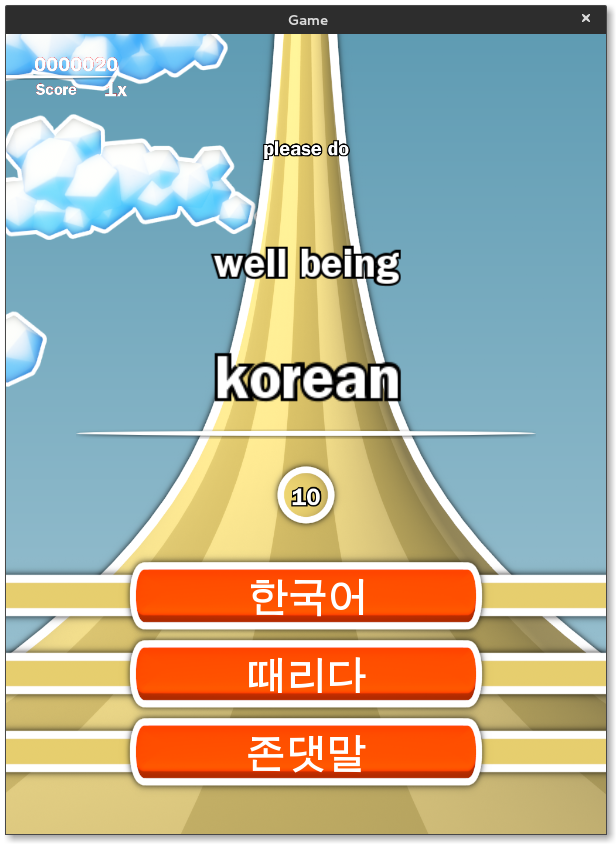
\includegraphics[width=5.5cm]{pic/defg-korean.png}
\end{center}
\caption{Primer delovanja Korejske verzije na namiznem računalniku}
\label{korean}
\end{figure} 


Ena izmed glavnih zahtev igre je izpis različnih pisav in posebnih znakov. Poleg prikazane verzije nemščina-angleščina, je bila aplikacija razvita tudi z idejo učenja jezikov, ki ne uporabljajo latinice. Slika [\ref{korean}] prikazuje primer učenja Korejščine. Aplikacije mora biti sposobna izrisovati velik nabor različnih abeced.

\begin{figure}
\begin{center}
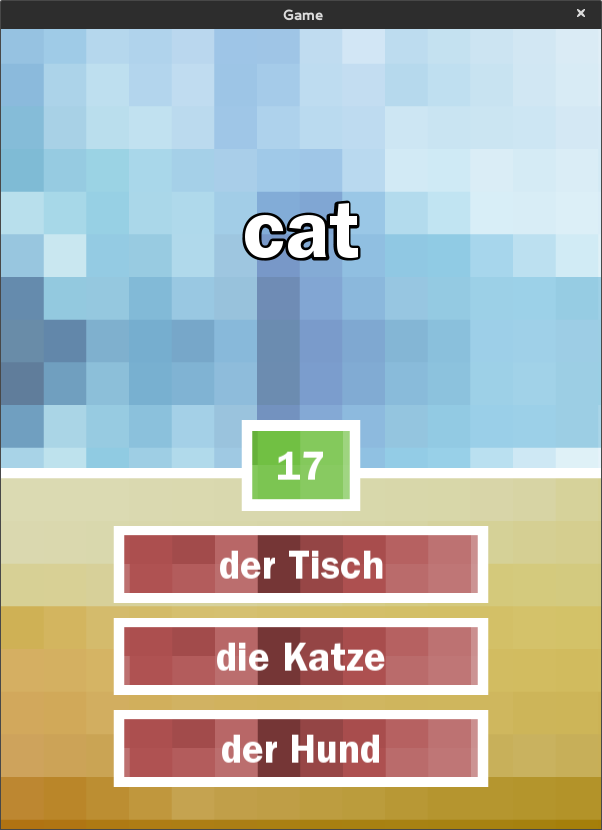
\includegraphics[width=5.5cm]{pic/defg-german.png}
\end{center}
\caption{Primer delovanja Nemške verzije na mobilni napravi}
\label{german}
\end{figure} 

Aplikacija je bila zamišljena kot mobilna aplikacijam za platformi iOS in Android, vendar kot smo že opisali je zelo uporabno imeti način razvoja na namiznem računalniku. Zaradi tega smo se odločili za metodo PlayN.

\subsection{Uporabljena metoda}

Izmed vseh obravnavanih metod se nam je zdela najbolj primerna metoda PlayN. Razlogi za izbiro PlayN so naslednji:

\begin{itemize}
\item PlayN je odprtokoden projekt. V primeru težav lahko pogledamo v izvorno kodo projekta in po potrebi nedelovanje spremenimo.
\item Licenca, ki jo PlayN uporablja, ni omejujoča in v primerjavi z nekaterimi plačljivimi metodami, ne zahteva nobenega plačila pred uporabo. To velja tudi, če bi aplikacijo namenili komercialnim namenom.
\item PlayN je še vedno v aktivnem razvoju, razvijalci pa so odzivni na listi za elektronsko pošto.
\item Orodje PlayN omogoča preprosto podporo dodajanju lastnih pisav, kar je ključnega pomena za podporo jezikom, kot je Korejščina.
\item Število platform, ki jih PlayN podpira, zadošča potrebam aplikacije.
\item PlayN omogoča uporabo vročega izmenjevanja kode, kar zelo pohitri razvoj aplikacije.
\item Poleg samega ogrodja PlayN je na voljo tudi precej vtičnikov, ki so jih napravili uporabniki. Tak primer je vtičnik Tripleplay, ki je v aplikaciji uporabljen za prikaz menijev.
\item Dokumentacija je dobro napisana in razumljiva.
\end{itemize}

Izbira je potekala med PlayN in podobno knjižnico LibGDX. Na koncu smo se odločili za PlayN zaradi lažje uporabe lastnih pisav v aplikaciji. O uporabi plačljivih rešitev nismo razmišljali.

\subsection{Opis metode}

Projekt z uporabo pogona PlayN sestavlja več imenikov. Glavni imenik se imenuje $core$ in vsebuje logiko celotne aplikacije. Izvorna koda, ki se nahaja v tem imeniku, definira kaj se bo na zaslonu prikazalo ter kako se aplikacija odziva na vnose uporabnikov. 

Imenik $assets$ služi kot imenik vseh sredstev, ki jih aplikacija potrebuje za delovanje. V imeniku se nahaja vsa grafika, ki je v uporabi v igri, in vse zvočne datoteke.

Ostali imeniki so namenjeni posameznim platformam. Imenik $java$ vsebuje preprost program, ki odpre okno in nastavi grafično okolje. Ko je okno pripravljeno pokliče glavno metodo imenika $core$ in aplikacija se začne izvajati. Slično delujeta tudi imenika $android$ in $ios$, vsak za svojo platformo. Oba definirata vse potrebno za zagon na sistemih Android in iOS in nato pokličeta metoda iz imenika $core$.



\subsection{Prednosti izbora metode}

Izbrana metoda nam je pomagala izpolniti vse zastavljene cilje. Brez truda smo aplikacijo razvijali na miznem računalniku in po potrebi preizkusili delovanje na Android napravi. Vmesnik API je razumljiv in krivulja učenja ni bila strma. 

\subsection{Slabosti izbora metode}

Težave smo imeli pri testiranju verzije za iOS naprave. Kljub izčrpni dokumentaciji smo naleteli na probleme, ki smo jih rešili samo s pomočjo odgovora na elektronski listi. 

Nekaj težav je povzročil tudi prehod na novo verzijo (1.6 in 1.7), ki se je zgodil med samim razvojem. Nova verzija je malce predrugačila način dela s sredstvi tako da smo naš projekt morali ročno popravljati.

\section{Primer štiri v vrsto}

Testna aplikacija je preprosta igra štiri v vrsto postavljena v treh dimenzijah. Ideja aplikacije je skozi preprosto igro izboljšati uporabnikovo orientacijo v 3D prostoru. Za razliko od standardne igre štiri v vrsto, kjer so zmagovalne kombinacije omejene v vodoravni, navpični in horizontalni smeri, imamo v 3D verziji veliko več možnosti. Poleg osnovnih smeri lahko zmagovalno kombinacijo zgradimo tudi v globino, kar odpre obilico novih kombinacij.

\subsection{Uporabljena metoda}

Za razvoj smo se odločili za orodje Unity. Unity za razliko od ostalih metod, ki smo se jih ogledali, Unity vključuje svoj urejevalnik. Urejevalnik nam omogoča grajenje objektov, postavitev kamere in določitev luči. Za postavitev objektov v 3D prostor se uporablja okno z ortografsko ali perspektivno projekcijo ter različnimi možnimi pogledi. 

S pomočjo uporabniškega vmesnika določimo pozicije objektov, materiale in druge lastnosti. Za logiko, obnašanje in odziv na uporabniški vhod pa vsakemu objektu lahko dodelimo tudi skriptno datoteko. V tej skriptni datoteki v enem od podprtih programskih jezikih (C\#, JavaScript, ??) določimo kako se bo objekt odzival na uporabniški vhod in določimo kako se bo obnašal v času, ko je viden na zaslonu.

\subsection{Prednosti metode}

Unity urejevalnik nam je omočil zelo hiter razvoj aplikacije, saj je bilo ustvarjanje osnovnih oblik in postavitev le teh v prostor, zelo preprosto. Pisanje skriptnih datotek za obnašanje in logiko aplikacije je bilo tudi preprosto.

\subsection{Slabosti metode}

Problem uporabe orodja Unity je učna krivulja. Za razliko od večine ostalih metod, se moramo poleg vmesnika API naučiti tudi dela s priloženim urejevalnikom. Sicer je urejevalnik preprost za uporabo, vendar učenje vseh potrebnih operacij vzame precej časa.

Druga slabost metode je v zaprtost sistema. Če tekom razvoja aplikacije naletimo na omejitev orodja nimamo dostopa do izvorne kode, kjer bi to omejitev lahko odpravili. Orodje je sicer na voljo brezplačno, vendar moramo za uporabo naprednih funkcij plačati za licenco. Aplikacije razvite z brezplačno verzijo programa imajo na vseh platformah pred zagonom zaslon z napisom Unity. 

Na sliki [\ref{mineditor}] je vidno kako poteka razvoj v okolju Unity.

\begin{figure}
\begin{center}
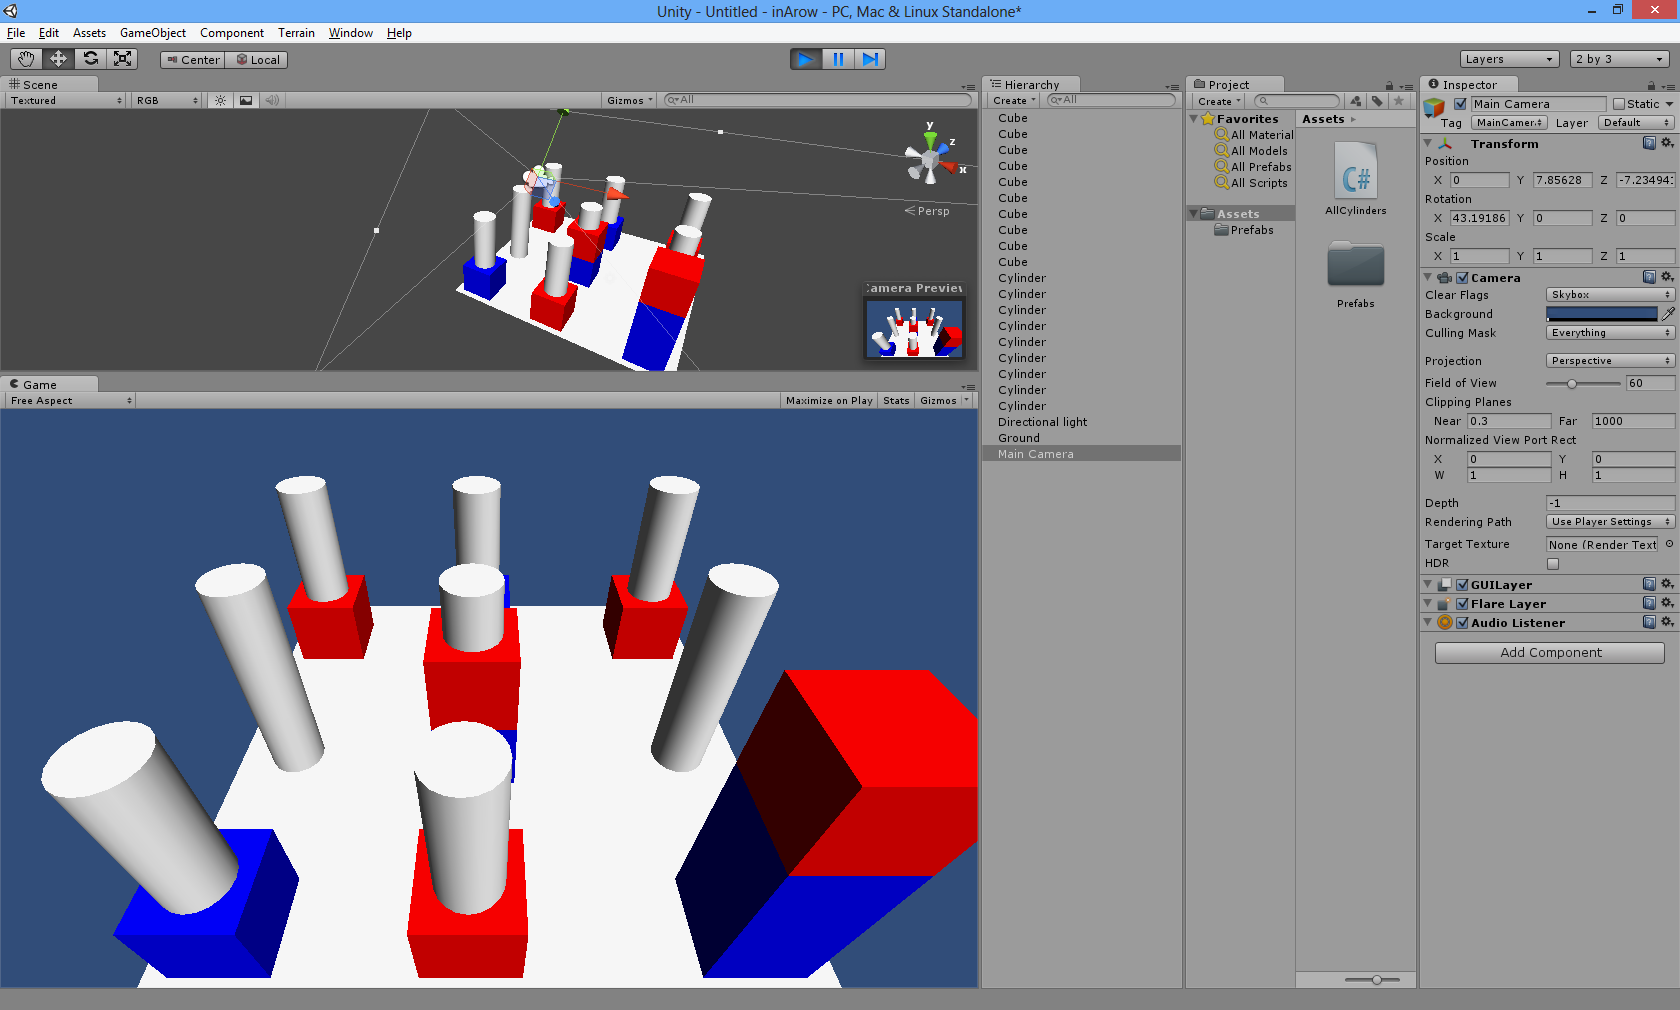
\includegraphics[width=12cm]{pic/min-editor.png}
\end{center}
\caption{Razvoj grafično intenzivne aplikacije v okolju Unity.}
\label{mineditor}
\end{figure} 

Slika \ref{minplay} prikazuje delovanje aplikacije na mobilni platformi Nexus 7.

\begin{figure}
\begin{center}
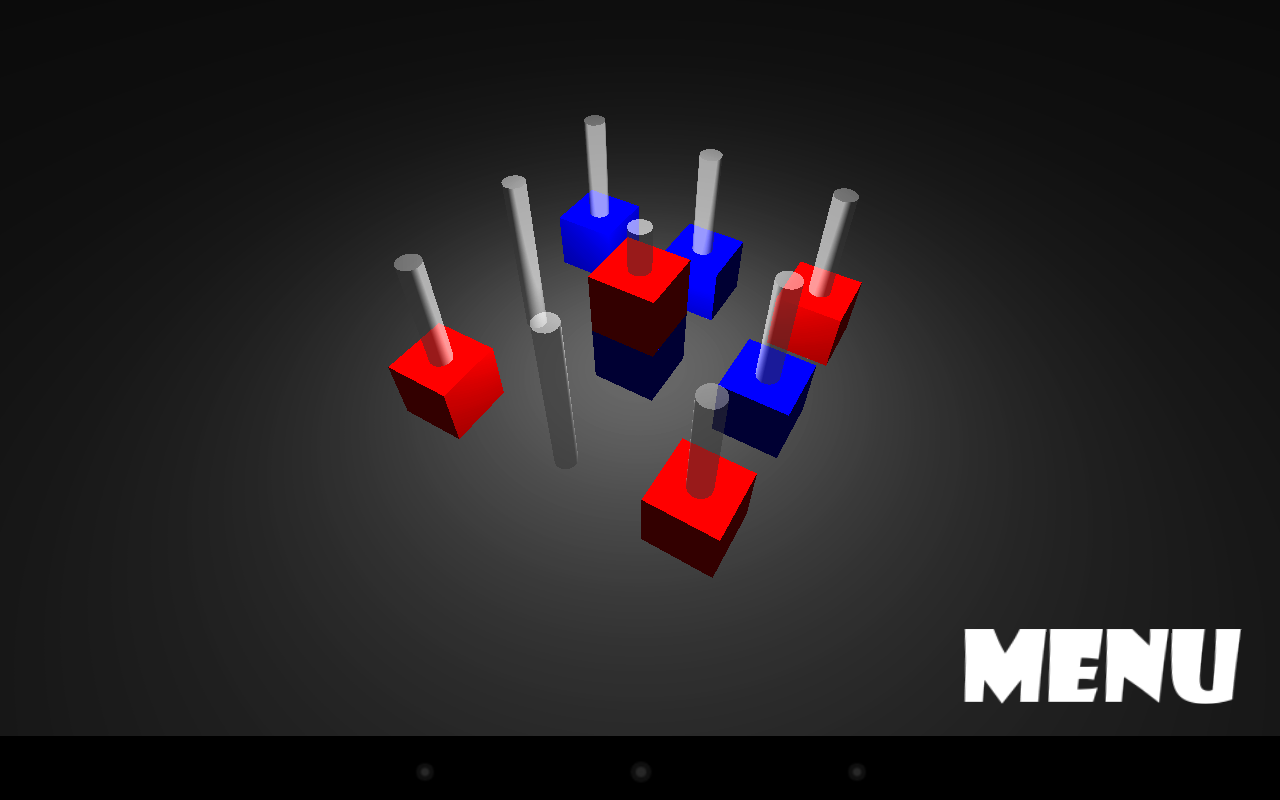
\includegraphics[width=10cm]{pic/min-play.png}
\end{center}
\caption{Končana Unity aplikacija izvožena na mobilno platformo.}
\label{minplay}
\end{figure} 

%\section{Primer C++}

%\section{Primer MIN}

%Primer Min je bil narejen s pomočjo knjižnice LibGDX. Za svoje delovanje izrablja %zmoglivosti OpenGL ES 2.0. 



\chapter{Sklepne ugotovitve}
Sklep.


\begin{thebibliography}{1}

% confirmed:

\bibitem{opengl} (Avgust, 2013) OpenGL Overview
\\ \url{http://www.opengl.org/about/}

\bibitem{direct3d} (Junij, 2013) Direct3D
\\ \url{http://msdn.microsoft.com/en-us/library/windows/desktop/hh309466(v=vs.85).aspx}

\bibitem{jezicno} Jure Dimec (2002), Medjezično iskanje dokumentov 
\\ \url{http://clir.craynaud.com/clir/MEDJEZICNOISKANJEDOKUMENTOV.pdf}

\bibitem{andriod} (Avgust, 2013) Android
\\ \url{http://www.android.com/}

\bibitem{ios} (Avgust, 2013) iOS
\\ \url{http://www.apple.com/ios/}

\bibitem{winphone} (Avgust, 2013) Windows Phone
\\ \url{http://developer.windowsphone.com/en-us}

\bibitem{angle} (Junij, 2013) ANGLE
\\ \url{https://code.google.com/p/angleproject/}

\bibitem{firefoxos} (Avgust, 2013) Firefox OS
\\ \url{http://www.mozilla.org/en-US/firefox/os/}

\bibitem{ubuntu} (Avgust, 2013) Ubuntu for phones
\\ \url{http://www.ubuntu.com/phone}

\bibitem{sailfishos} (Avgust, 2013) Sailfish OS
\\ \url{https://sailfishos.org/}

\bibitem{rasPi} (Avgust, 2013) Rasperry Pi FAQ
\\ \url{http://www.raspberrypi.org/faqs}

\bibitem{beagleBone} (Avgust, 2013) Beagle Bone
\\ \url{http://beagleboard.org/bone}

\bibitem{canvas} (Avgust, 2013) HTML Canvas 2D Context
\\ \url{http://www.w3.org/wiki/HTML/Elements/canvas}

\bibitem{webgl} (Avgust, 2013) OpenGL ES 2.0 for the Web 
\\ \url{http://www.khronos.org/webgl/}

\bibitem{soundjs} (Avgust, 2013) SoundJS
\\ \url{http://www.createjs.com/\#!/SoundJS}

\bibitem{jsperformance} Michael Mahemoff (Junij, 2011), HTML5 vs Native: The Mobile App Debate
\\ \url{http://www.html5rocks.com/en/mobile/nativedebate/}

\bibitem{v8gl} (Avgust, 2013) V8-GL 
\\ \url{https://github.com/philogb/v8-gl}

\bibitem{lycheejs} (Avgust, 2013) LeechyJS 
\\ \url{http://martens.ms/lycheeJS/}

\bibitem{xamarin} (Avgust, 2013) Xamarin
\\ \url{http://xamarin.com/}

\bibitem{libgdx} (Avgust, 2013) LibGDX 
\\ \url{http://libgdx.badlogicgames.com/}

\bibitem{ikvm} (Februar, 2013) IKVM.NET
\\ \url{http://www.ikvm.net/}

\bibitem{playn} (Avgust, 2013) PlayN 
\\ \url{http://code.google.com/p/playn/}

\bibitem{mvn} (Avgust, 2013) Apache Maven Project
\\ \url{http://maven.apache.org/}

\bibitem{unity} (Avgust, 2013) Unity - Game engine, tools and mulitplatform
\\ \url{http://unity3d.com/unity/}

\bibitem{haxe} (Avgust, 2013) Haxe Documentation
\\ \url{http://haxe.org/}

\bibitem{gameplay} (Avgust, 2013) Gameplay Overview
\\ \url{http://www.gameplay3d.org/}

\bibitem{ogre} (Avgust, 2013) OGRE - Open Source 3D Graphics Engine
\\ \url{http://www.ogre3d.org}

\bibitem{marmalade} (Avgust, 2013) Marmalade
\\ \url{http://www.madewithmarmalade.com/}

\bibitem{flash} (Avgust, 2013) Adobe Flash
\\ \url{http://www.adobe.com/products/flash.html}

\bibitem{asm} (Avgust, 2013) asm.js
\\ \url{http://asmjs.org/}

\bibitem{cuda} (Avgust, 2013) What is CUDA
\\ \url{https://developer.nvidia.com/what-cuda}

\bibitem{cuda-mobile}  Jonah Alben (Julij, 2013), CUDA na mobilnih napravah
\\ \url{http://blogs.nvidia.com/blog/2013/07/24/kepler-to-mobile/}

\bibitem{opencl} (Avgust, 2013) The open standard for parallel programming of heterogeneous systems
\\ \url{http://www.khronos.org/opencl/}

\bibitem{accelereyes} (Avgust, 2013) AccelerEyes
\\ \url{http://www.accelereyes.com/products/mobile}

\bibitem{lwjgl} (Avgust, 2013) LWJGL Lightweight Java Game Library
\\ \url{http://www.lwjgl.org/}

\end{thebibliography}


%\begin{thebibliography}{99}
%\bibitem{lf} L.\ Fortnow, ``Viewpoint: Time for computer science to grow up'',
%{\it Communications of the ACM}, št.\ 52, zv.\ 8, str.\ 33--35, 2009.
%\bibitem{dk1} D.\ E.\ Knuth, P. Bendix. ``Simple word problems in universal algebras'', v zborniku: Computational Problems in Abstract Algebra (ur. J. Leech), 1970, str. 263--297.
%\bibitem{lat} L.\ Lamport. {\it LaTEX: A Document Preparation System}. Addison-Wesley, 1986.
%\bibitem{bib} O.\ Patashnik (1998) \BibTeX{}ing. 
%\\ http://ftp.univie.ac.at/packages/tex/biblio/bibtex/contrib/doc/btxdoc.pdf
%\bibitem{licence} licence-cc.pdf. Dostopno na: 
%\end{thebibliography}



\end{document}

